\documentclass{esg8012pset}
\begin{preamble}
  \usepackage{amsmath}
  \usepackage{amssymb}
  \usepackage{enumerate}
  \usepackage{graphicx}
  \providecommand{\uvec}[1]{{\hat{\bf{#1}}}}
\end{preamble}

\classname{Physics 8.012}
\semester{Fall 2010}
\problemsetnumber{2}
\date{September 17}
\duedate{Friday, September 24}
\readingassignment{Kleppner and Kolenkow, \emph{An Introduction to Mechanics}, Chapter Two}
\begin{document}

\begin{question}[Problem 2]
\begin{problem}
  The two blocks shown in the figure are connected by a string of negligible mass. If the system is released from rest, find how far the block of mass $m_1$ slides in time $t$. Neglect friction.
  \begin{center}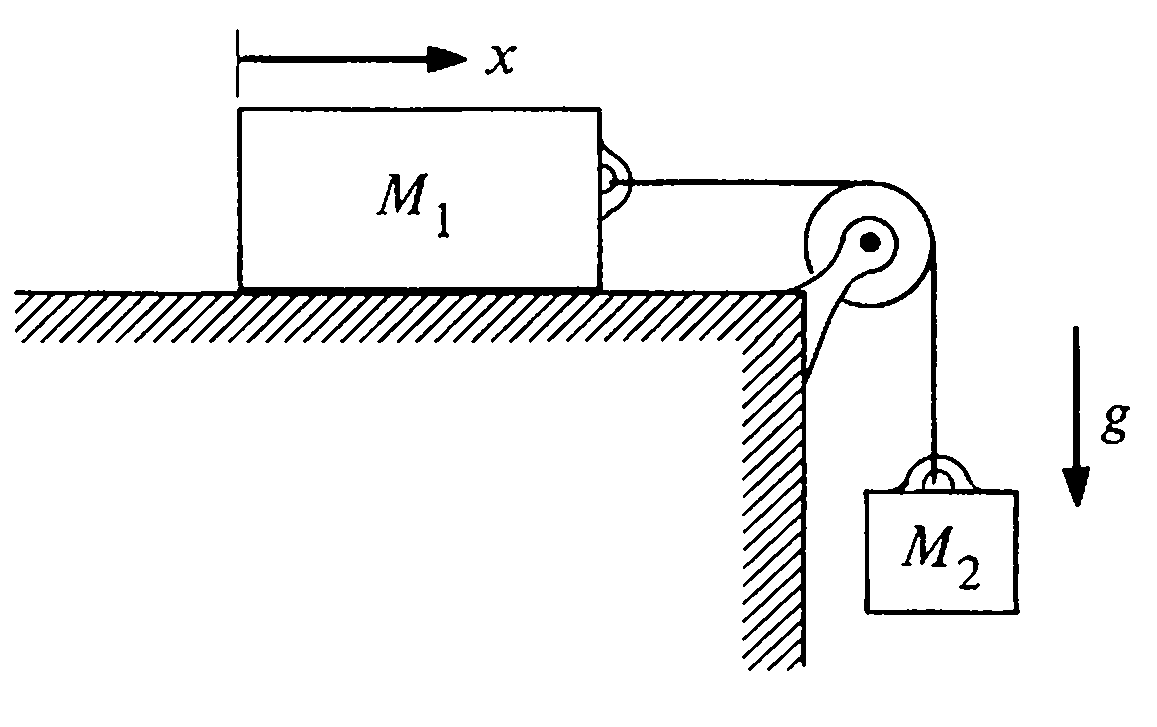
\includegraphics[width=0.35\textwidth]{ps02_1}\end{center}
\end{problem}
\begin{solution}
  The system can be treated as a single block of mass $m_1 + m_2$, with a force due to gravity of $m_2 g$.  The acceleration is then $\frac{m_2 g}{m_1 + m_2}$, so the distance is $\frac{m_2 g}{2(m_1 + m_2)} t^2$.
\end{solution}
\end{problem}


\section*{Problem 4}
\subsection*{Problem} Two particles of mass $m_1$ and $m_2$ undergo uniform circular motion about each other at a separation $R$ under the influence of an attractive force of magnitude $F$.  The angular velocity is $\omega$ radians per second.
\begin{enumerate}[a)]
  \item Show that $R = \left(\frac{F}{\omega^2}\right)\left(\frac{1}{m_1} + \frac{1}{m_2}\right)$.
  \item Explain why you can think of this problem is equivalent to a single body of mass $\mu$ where $\frac{1}{\mu} = \left(\frac{1}{m_1} + \frac{1}{m_2}\right)$ undergoing circular motion of radius $R$ due to the influence of a central attractive force of magnitude $F$.
\end{enumerate}
\subsection*{Solution}
\begin{enumerate}[a)]
  \item Let $r_1$ and $r_2$ denote the radii of the circles of $m_1$ and $m_2$, respectively.  Then $R = r_1 + r_2$.  Since the movement is uniform and circular, the force must be $\frac{m_1 v_1^2}{r_1} = \frac{m_2 v_2^2}{r_2}$.  The acceleration of $m_1$ is then $\frac{v_1^2}{r_1}$, and the acceleration of $m_2$ is $\frac{v_2^2}{r_2}$.  Since the angular velocity is $\omega$, and the circumference is $2\pi r_1$ and $2\pi r_2$, respectively, $v_1 = \frac{2\pi r_1}{\frac{2\pi}{\omega}} = r_1 \omega$ and $v_2 = r_2 \omega$.  Then $F = m_1 r_1 \omega^2 =  m_2 r_2 \omega^2$.  Since $R = r_1 + r_2$, $F = m_1 r_1 \omega^2 = m_2 (R - r_1) \omega^2$.  So $F = m_1 r_1 \omega^2 = m_2 R \omega^2 - m_2 r_1 \omega^2$.  Dropping the $F$, $m_1 r_1 = m_2 R - m_2 r_1$, so $(m_1 + m_2)r_1 = m_2 R$.  Then $r_1 = \frac{R m_2}{m_1 + m_2}$.  Thus, $F =  \frac{R m_1 m_2\omega^2}{m_1 + m_2}$, so $R = \frac{F(m_1+m_2)}{\omega^2 m_1 m_2} = \frac{F}{\omega^2}\left(\frac{1}{m_1}+\frac{1}{m_2}\right)$.
  \item Let $\vec r_{AB} = \vec r_B - \vec r_A$ as shown below. \begin{center}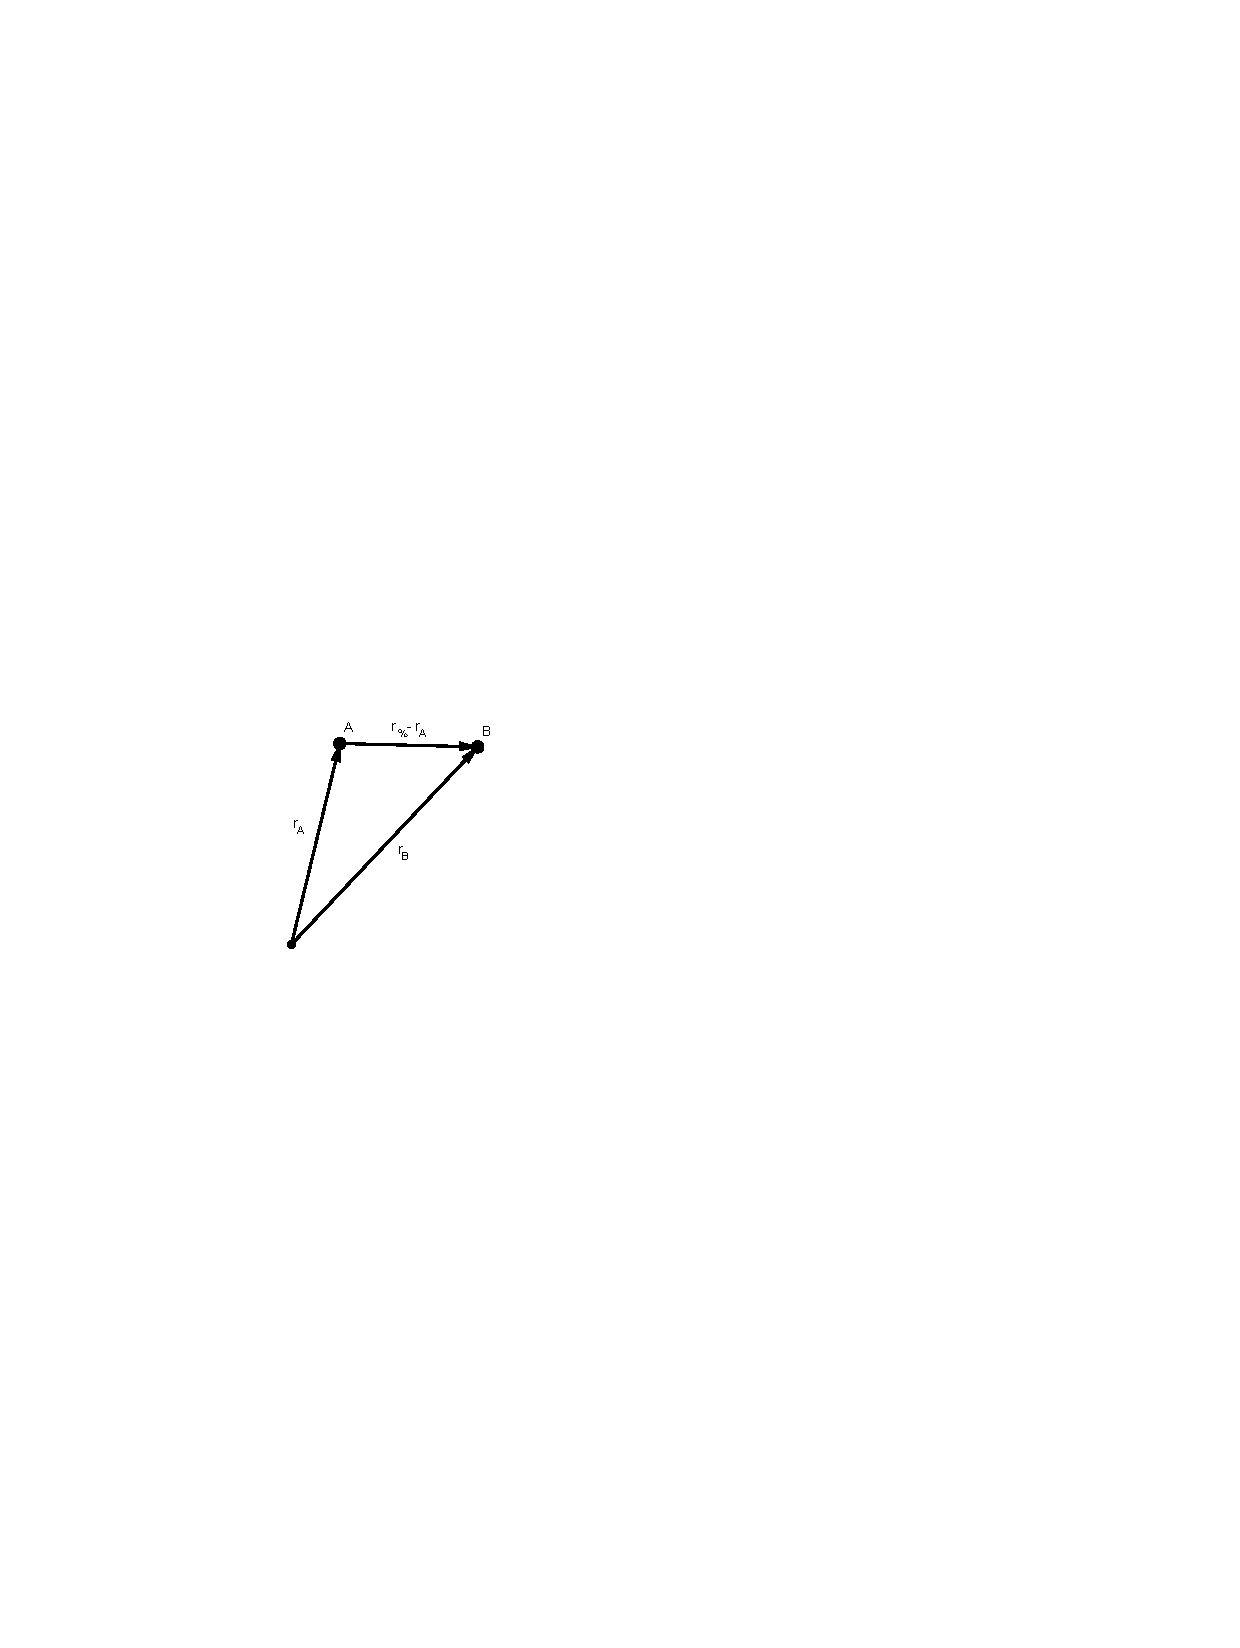
\includegraphics[width=0.5\textwidth]{2009-09-25_Diagram_10}\end{center}  Then $\vec F_{AB} = m_B \vec a_B$ and $\vec F_{BA} = m_A \vec a_A = -\vec F_{AB}$.  $\frac{\vec F_{AB}}{m_B} - \frac{\vec F_{BA}}{m_A} = \vec a_B - \vec a_A$, so $\vec F_{AB}\left(\frac{1}{m_A} + \frac{1}{m_B}\right) = \frac{\partial^2}{\partial t^2}(\vec r_B - \vec r_A)$.  Then $\vec F_{AB}\left(\frac{1}{m_A} + \frac{1}{m_B}\right) = \frac{\partial^2}{\partial t^2}\vec r_{AB}$.  Define $\mu$ such that $\frac{1}{\mu} = \frac{1}{m_A} + \frac{1}{m_B}$, and $\omega$ to be $\left\vert \frac{\partial \hat r_{AB}}{\partial t}\right\vert$.  Then $\vec F_{AB} = \mu \frac{\partial^2}{\partial t^2}\vec r_{AB} = -\mu R\omega^2\hat r_{AB}$, since the vector is rotating with uniform angular momentum.  Then $R = \frac{F}{\omega^2}\mu$, which corresponds to the setup in (a).
\end{enumerate}

\section*{Problem 7}
\subsection*{Problem} Consider two textbooks that are resting one on top of the other. The lower book has $m_2 = 0.8$ kg and is resting on a nearly frictionless surface. The upper book has mass $m_1 = 2.0$ kg. Suppose the coefficient of static friction is given by $\mu_s = 0.1$.
\begin{center}\includegraphics{2009-09-25_ps02_2}\end{center}
\begin{enumerate}[a)]
  \item What is the maximum force which the upper book can be pushed horizontally so that the two books move together without slipping? Identify all action-reaction pairs of forces in this problem.
  \item What is the maximum force which the lower book can be pushed horizontally so that the two books move together without slipping? Identify all action-reaction pairs of forces in this problem.
  \item Explain why one of your forces in parts a) and b) is larger than the other.
\end{enumerate}
\subsection*{Solution}
\begin{enumerate}[a)]
  \item The top block exerts friction on the bottom block, and vice versa.  Gravity exerts a force on each block, and the surface below exerts a normal force.  The blocks can be treated as a single block with mass $m_1 + m_2$ to which $F_{\text{applied}}$ is applied.  The acceleration is $\frac{F_{\text{applied}}}{m_1 + m_2}$.  The maximal force due to friction is $\mu_s F_n = m_1 g \mu_s$.  The maximal acceleration of the top block is thus $\frac{\mu_s m_1 g}{m_1} = \mu_s g = 1$ m / s$^2$.  Thus, the maximal applied force is $(1\text{ m / s}^2)(m_1 + m_2) = 3$ N.
    \par\begin{center}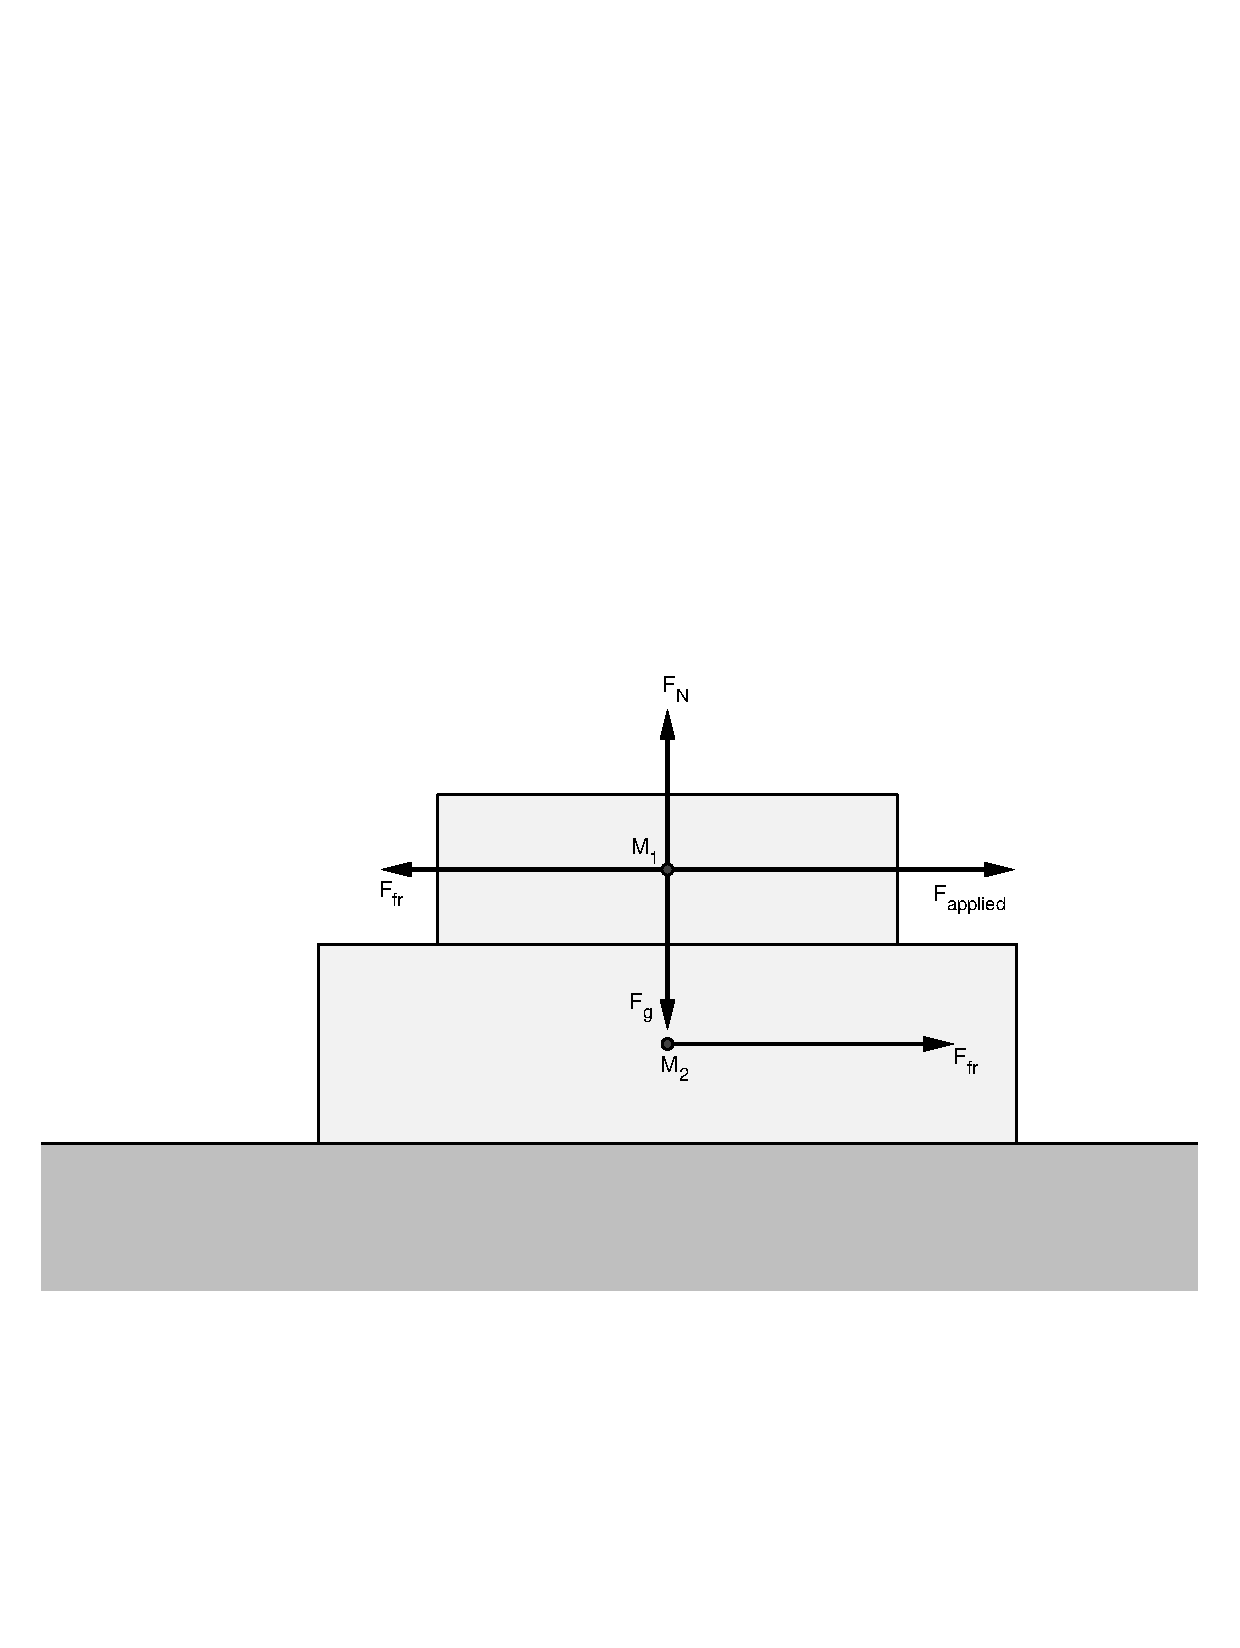
\includegraphics[width=0.5\textwidth]{2009-09-25_Diagram_2}\end{center}
  \item The top block exerts friction on the bottom block, and vice versa.  Gravity exerts a force on each block, and the surface below exerts a normal force.  The blocks can be treated as a single block with mass $m_1 + m_2$ to which $F_{\text{applied}}$ is applied.  The acceleration is $\frac{F_{\text{applied}}}{m_1 + m_2}$.  The maximal force due to friction is $\mu_s F_n = m_1 g \mu_s$.  The maximal acceleration of the top block is thus $\frac{\mu_s m_1 g}{m_2} = 2.45\text{ m / s}^2\approx 2$ m / s$^2$.  Thus, the maximal applied force is $(2\text{ m / s}^2)(m_1 + m_2) = 7$ N.
    \par\begin{center}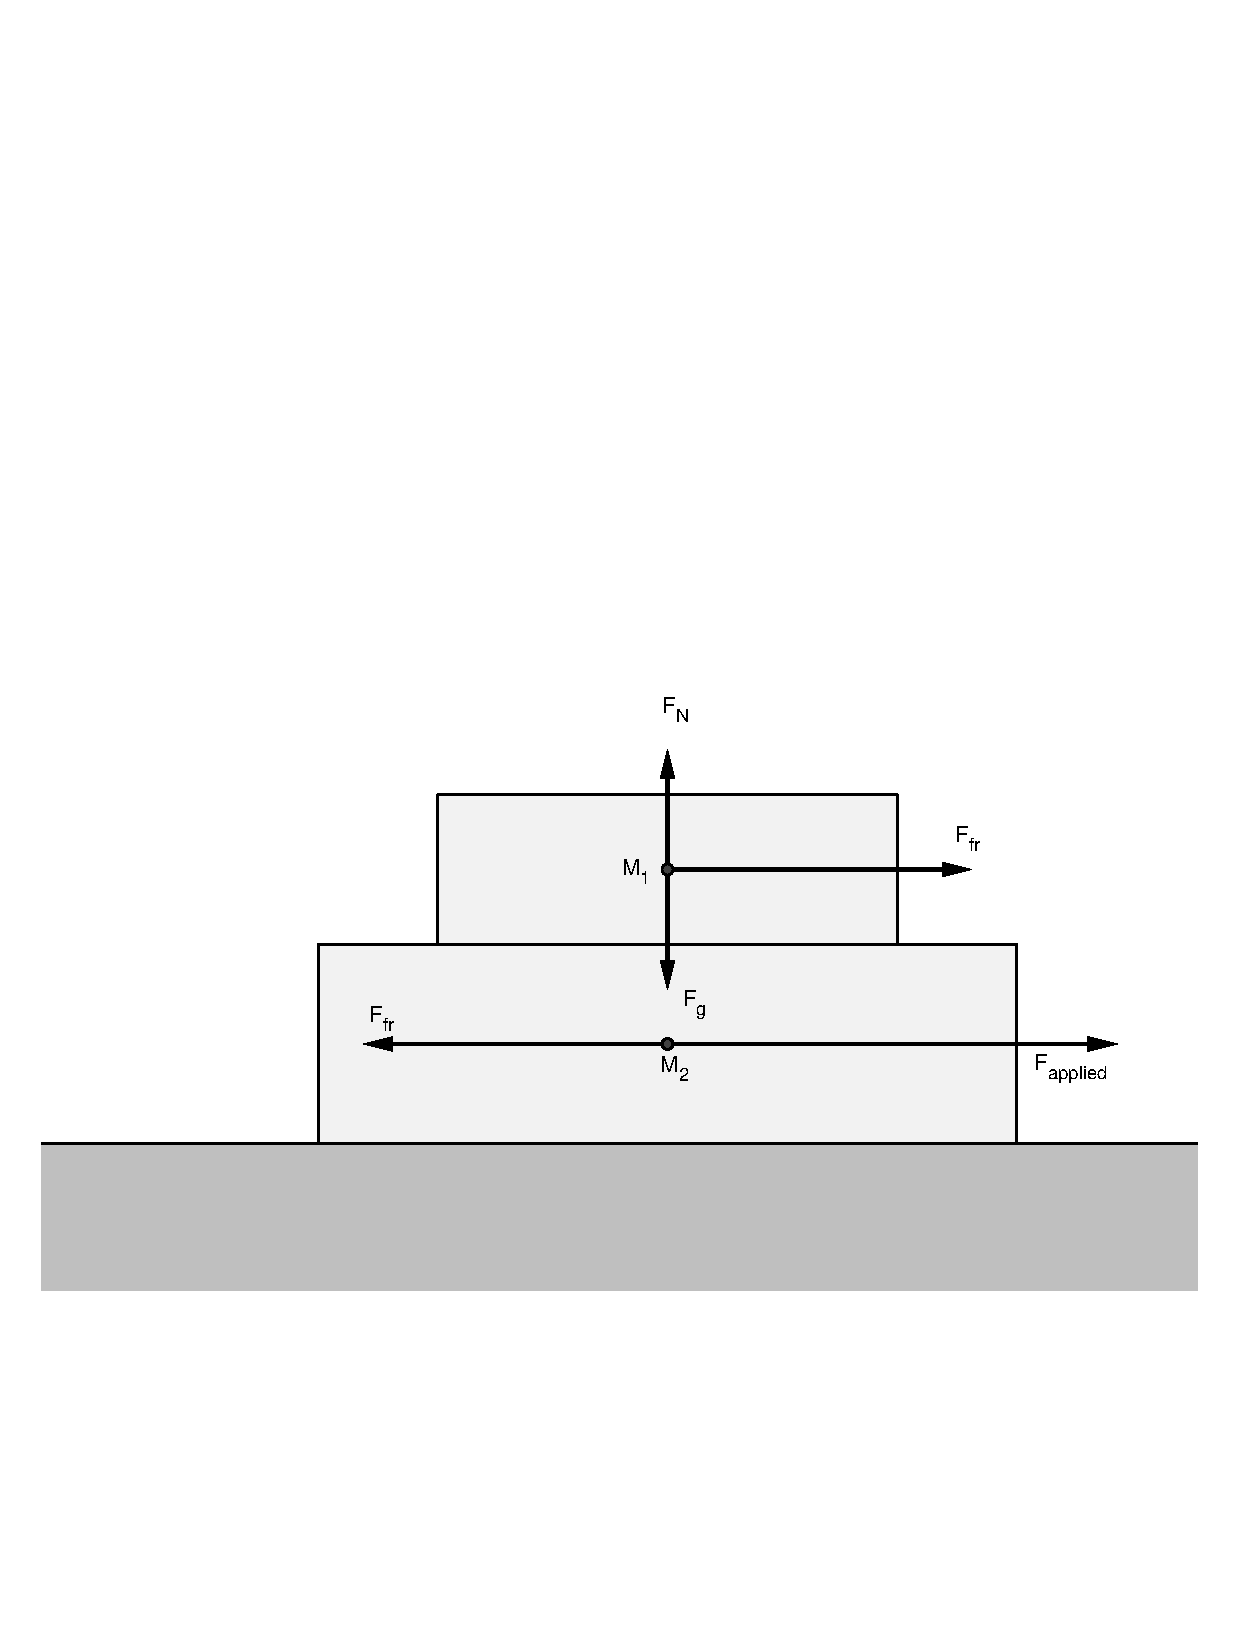
\includegraphics[width=0.5\textwidth]{2009-09-25_Diagram_1}\end{center}
  \item The maximal acceleration due to friction is the same in both cases, but the acceleration is of a larger mass in part b), so more force can be applied.
\end{enumerate}

\section*{Problem KK 2.9}
\subsection*{Problem} A body of mass $m$ is moving in a horizontal circle of radius $r$ with a constant speed $v_0$ on the inside wall of a cone. Assume the wall of the cone is frictionless. The wall of the cone makes an angle $\theta$ with the vertical.
\begin{center}\includegraphics{2009-09-25_ps02_3}\end{center}
\begin{enumerate}[a)]
  \item Draw a free body force diagram showing all the forces acting on the mass.
  \item What is the speed of the mass?
  \item How long will the mass take to go around the circle?
  \item Now assume there is a coefficient of static friction $\mu_s$. Find the maximum speed the mass can move on the inside of a cone and still move in a circular orbit of radius $r$.
\end{enumerate}
\subsection*{Solution}
\begin{enumerate}[a)]
  \item \hfil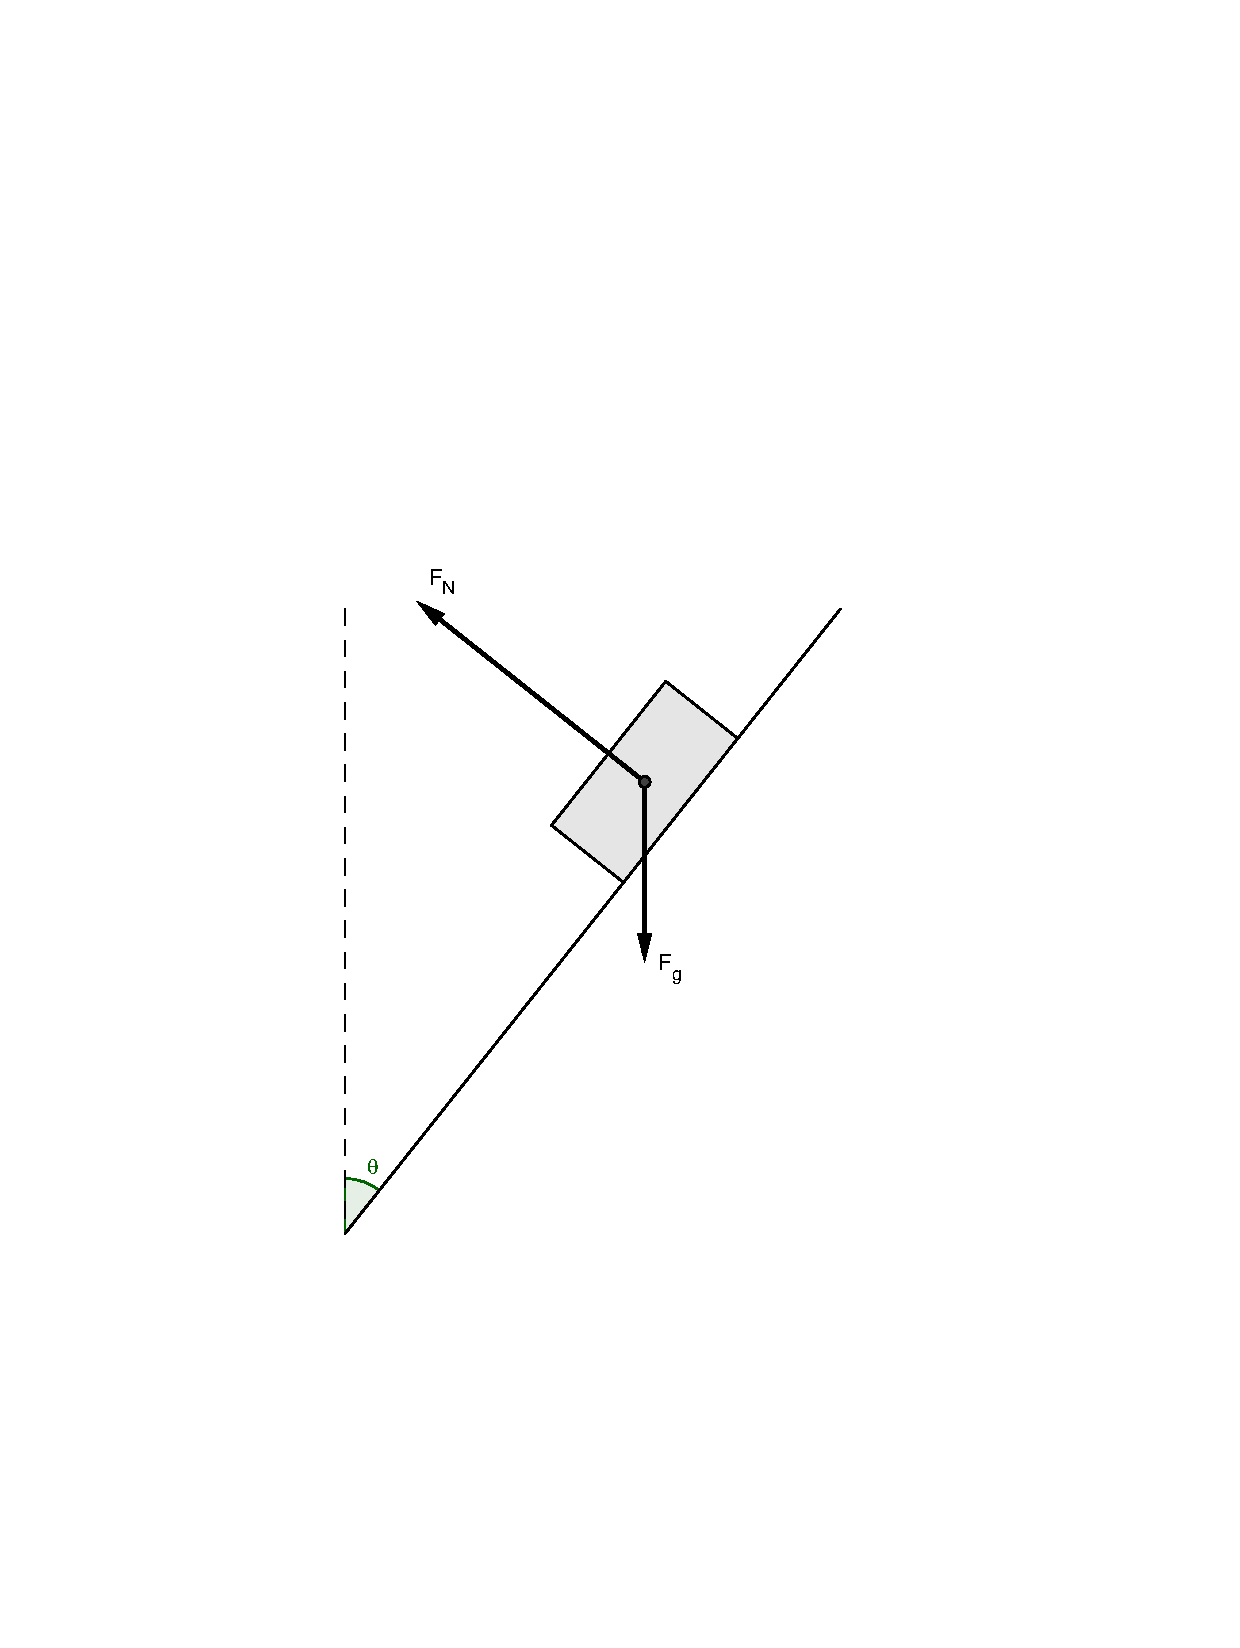
\includegraphics[width=0.25\textwidth]{2009-09-25_Diagram_3}\hfil
  \item For circular motion, $\frac{\partial \vec r}{\partial t} = r\frac{\partial \theta}{\partial t}\hat \theta = v_0 \hat \theta$, so $\frac{\partial^2 \vec r}{\partial t^2} = -r\left(\frac{\partial \theta}{\partial t}\right)^2\hat r = -\frac{v_0^2}{r}\hat r$.  Since $F_N\sin\theta = mg$, and $\vec F_{\text{net}} = -F_N\cos\theta\hat i$, $\frac{mg}{\sin\theta}\cos\theta = m\frac{v_0^2}{r}$, so $v_0 = \sqrt{gr\cot\theta}$.
  \item The circumference is $2\pi r$, and $v_0 = \sqrt{gr\cot\theta}$, so it takes $\frac{2\pi\sqrt{r}}{\sqrt{g\cot\theta}}$.
  \item FIX The diagram becomes: \begin{center}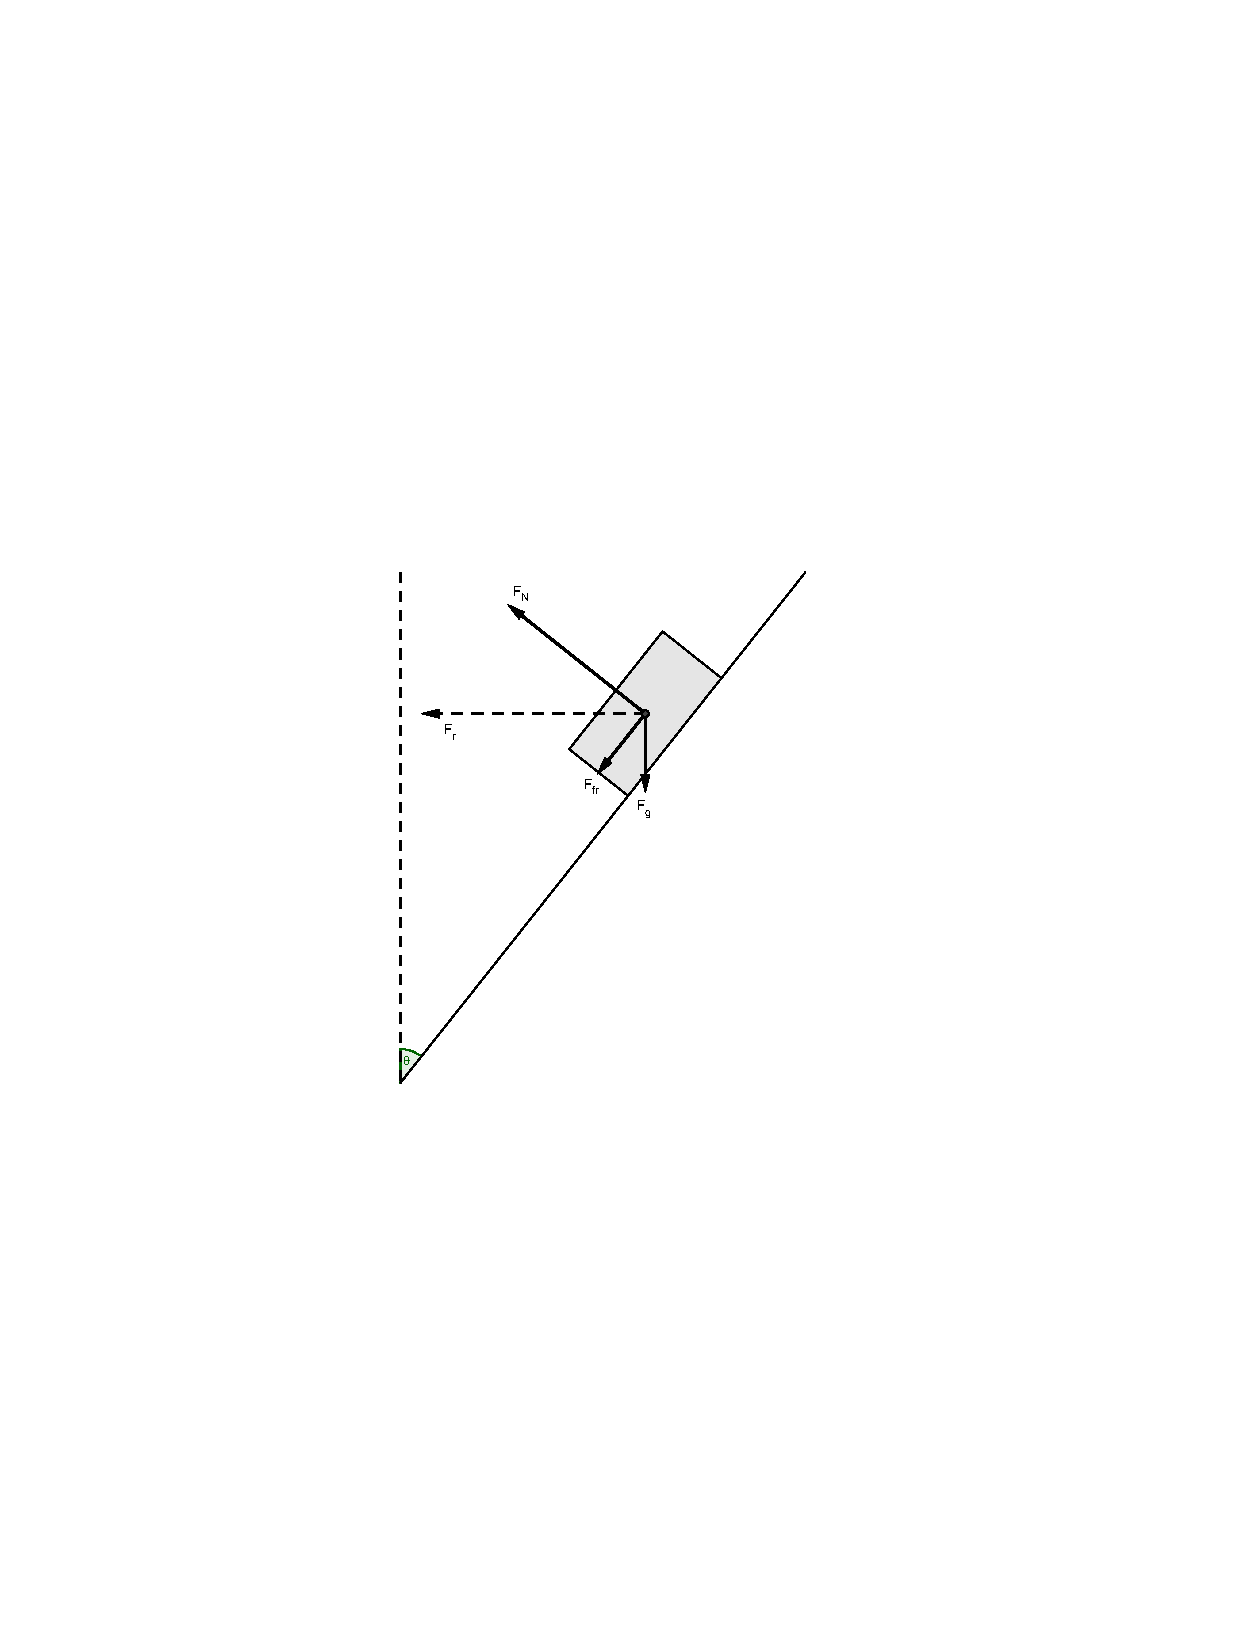
\includegraphics[width=0.25\textwidth]{2009-09-25_Diagram_8}\end{center}  Decomposing the vectors, \begin{center}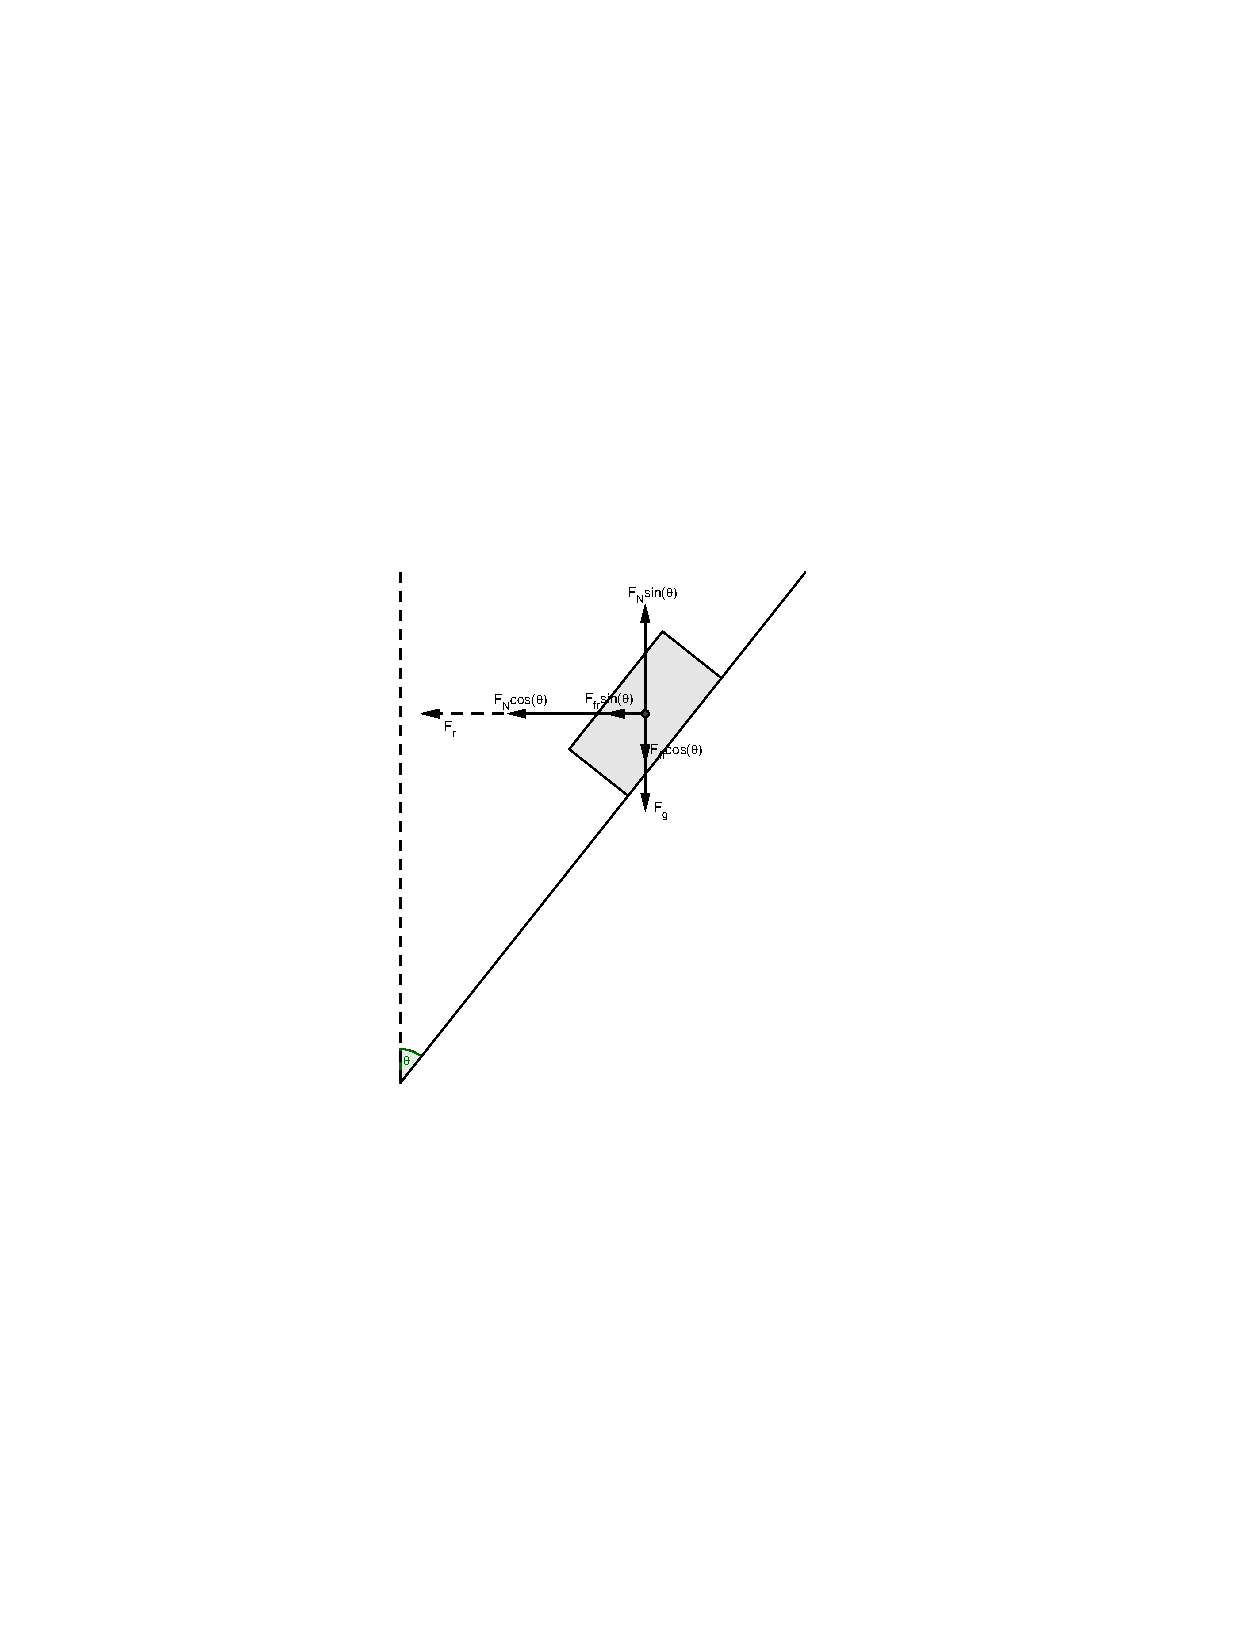
\includegraphics[width=0.25\textwidth]{2009-09-25_Diagram_9}\end{center}  The radial acceleration is $\frac{v^2}{r}$, so $\frac{\partial^2 \vec r}{\partial t^2} = -\frac{v^2}{r}\hat i$.  Then $m\frac{v^2}{r} = F_{\text{fr}}\sin\theta + F_g\cos\theta = F_N \mu_s + F_g\cos\theta$.  The normal force is $m\frac{v^2}{r}\cos\theta$.  Then $m\frac{v^2}{r} = m\frac{v^2}{r}\cos\theta \mu_s + mg\cos\theta$, so $\frac{v^2}{r}(1 - \cos\theta \mu_s) = g\cos\theta$, so $v = \sqrt{\frac{rg\cos\theta}{1-\cos\theta\mu_s}}$. ???
\end{enumerate}

\section*{Problem 2.10}
\subsection*{Problem} The earth is spinning about its axis with a period of 23 hours 56 min and 4 sec. The equatorial radius of the earth is $6.38\cdot 10^{6}$ m. The latitude of Cambridge, Mass is 42$^{\circ}$ 22'.
\begin{enumerate}[a)]
  \item Find the velocity of a person at MIT as they undergo circular motion about the earth? axis of rotation.
  \item Find the person's centripetal acceleration.
  \item The rotation of the Earth is slowing down. In 1977, the Earth took 1.01s longer to complete 365 rotations than in 1990. What was the average angular deceleration of the Earth in the time interval from 1900 to 1977?
  \item Find the radius of the orbit of a synchronous satellite which circles the earth. (A synchronous satellite goes around the earth once every rotation of the earth, so that its position appears stationary with respect to a ground station).
\end{enumerate}
\subsection*{Solution}
\begin{enumerate}[a)]
  \item The radius of the circle of rotation is $r_E \cos(42^{\circ} 22') \approx 4710$ km.  The circumference is then about 29600 km.  The velocity is thus $\frac{29600\text{ km}}{23\text{ h }56\text{ m }4\text{ s}} \approx 343$ m/s.
  \item The centripetal acceleration is $\frac{v^2}{r} \approx 0.0251$ m / s$^2$.
  \item The angular velocity is $\frac{2\pi}{t}$, so the angular deceleration is $\frac{\frac{365\cdot 2\pi}{1\text{ year}} - \frac{365\cdot 2\pi}{1\text{ year}+1.01\text{ s}}}{77\text{ years}} \approx 10^{-21}$ s$^{-2}$. 
  \item Since $v = \frac{2\pi r}{t}$, $a = G\frac{m_e}{r^2} = \frac{4\pi^2 r}{t^2}$, so $r = \sqrt[3]{\frac{G t^2}{4\pi^2}} \approx 42000$ km.
\end{enumerate}

\section*{Problem 2.16}
\subsection*{Problem} A 45$^{\circ}$ wedge is pushed along a table with constant acceleration $A$. A block of mass $m$ slides without friction down the wedge. Find its acceleration. (Gravity is directed down.)
\begin{center}\includegraphics{2009-09-25_ps02_4}\end{center}
\subsection*{Solution}
We begin with a coordinate transformation, substituting the acceleration of the wedge, $\vec A$, with a force in the opposite direction, $\vec F_A = -m \vec A$.
\begin{center}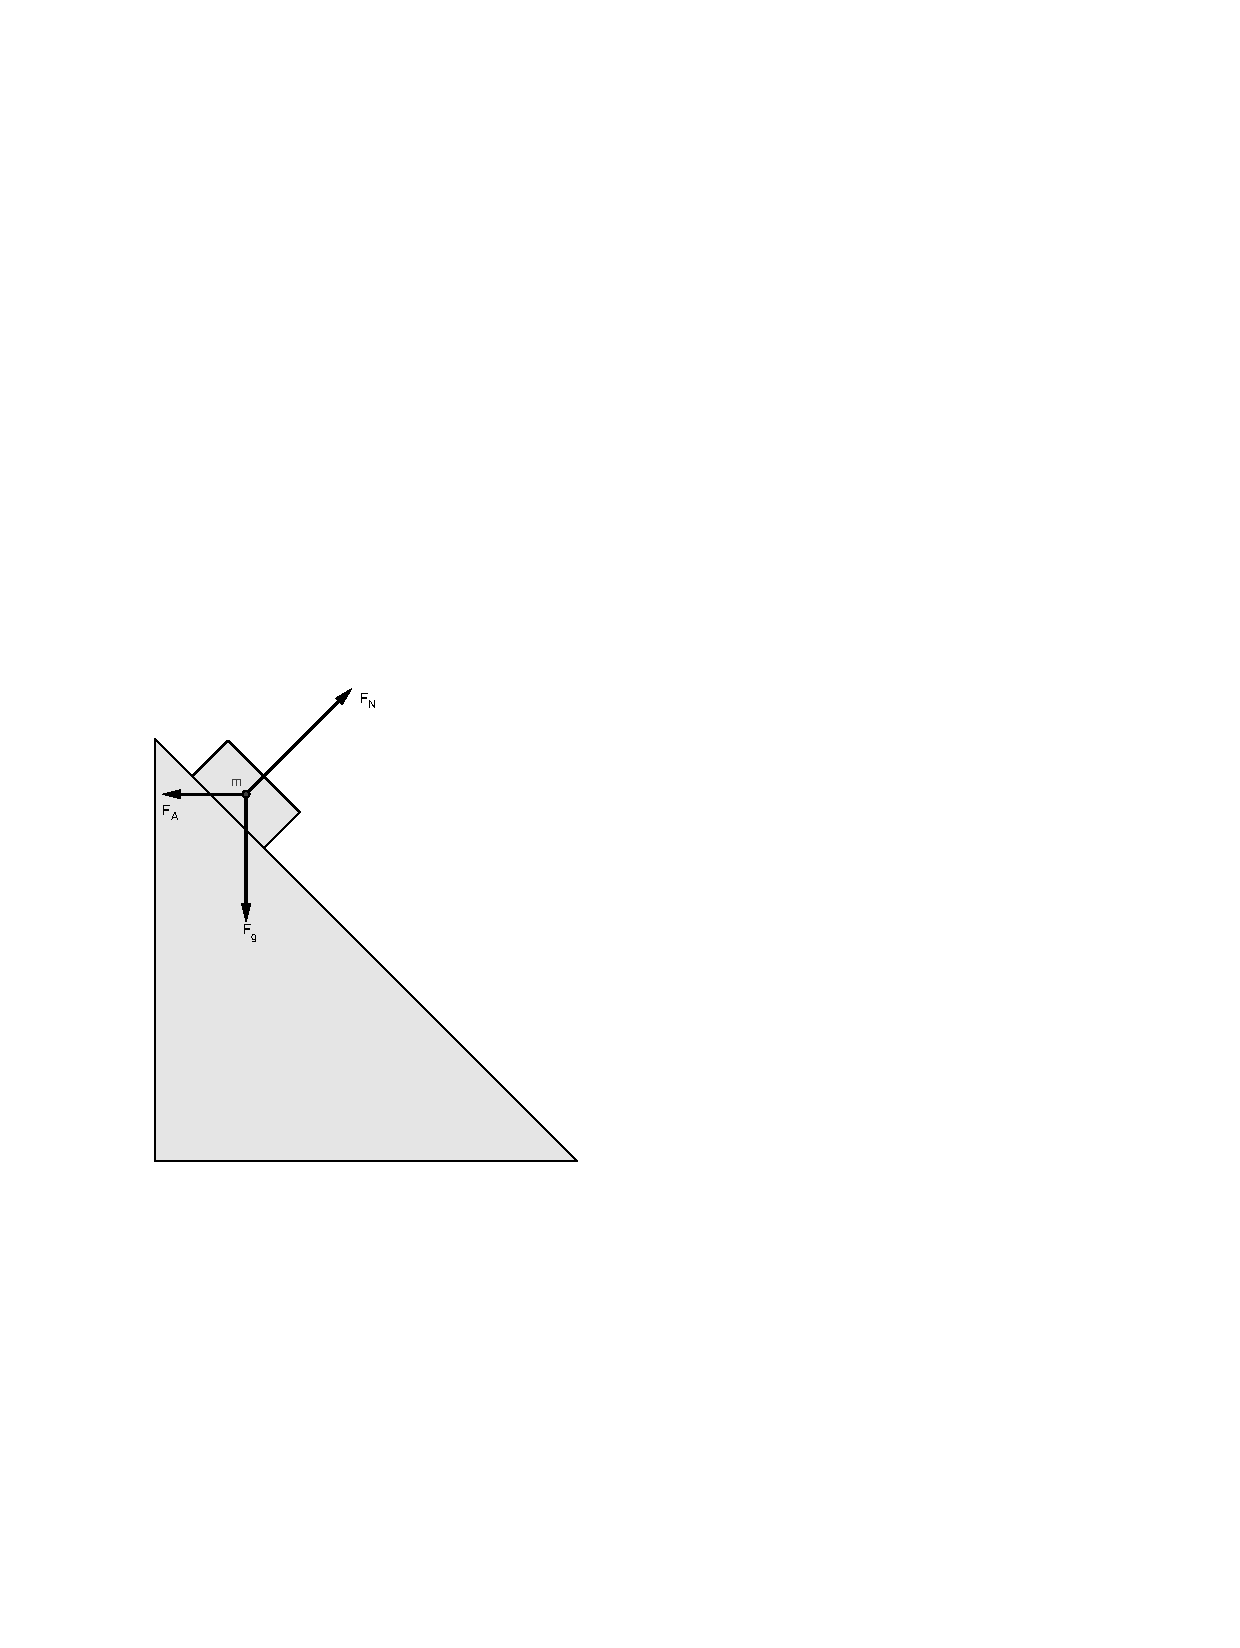
\includegraphics[width=.5\textwidth]{2009-09-25_Diagram_5}\end{center}
Decomposing the vectors, we get the following.
\begin{center}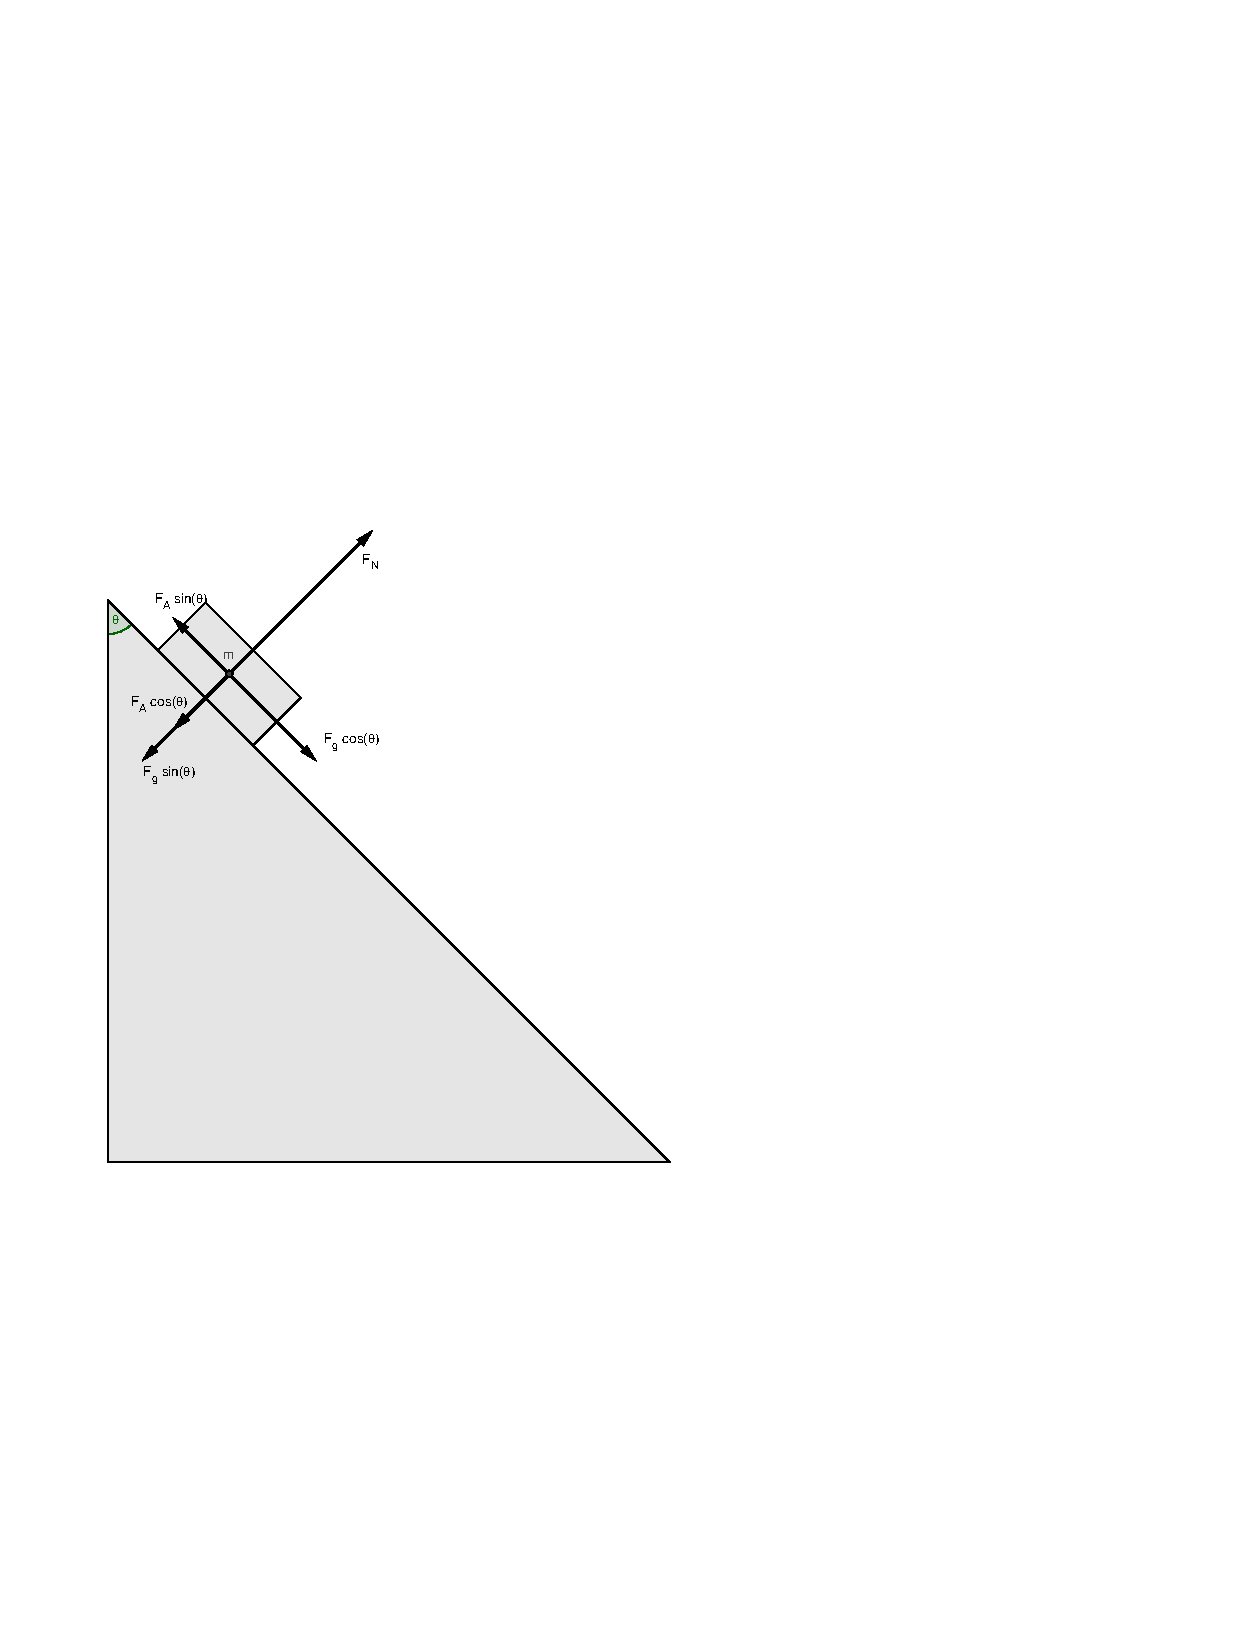
\includegraphics[width=.5\textwidth]{2009-09-25_Diagram_6}\end{center}

Since $\sin(45^{\circ}) = \cos(45^{\circ}) = \frac{1}{\sqrt{2}}$, the magnitude of the net force is $\frac{1}{\sqrt{2}}(F_g - F_A)$ down the wedge.  Then the acceleration is $\frac{1}{\sqrt{2}}(g - A)$ down the wedge.  Transforming back to the original coordinate system, the net acceleration is $A \hat i + \frac{1}{\sqrt{2}}(g - A)\left(\frac{1}{\sqrt{2}}\hat i - \frac{1}{\sqrt{2}} \hat j\right) = \frac{1}{2}(g + A) \hat i - \frac{1}{2}(g - A)\hat j$.

%The normal force of the wedge on the block, $F_n$, opposes the 

{\textbf{Alternative Solution:}}

\section*{Problem 2.22}
\subsection*{Problem} Suppose a rope of mass $m$ hangs between two trees. The ends of the rope are at the same height and they make an angle $\theta$ with the trees.
\begin{center}\includegraphics{2009-09-25_ps02_5}\end{center}
\begin{enumerate}[a)]
  \item What is the tension at the ends of the rope where it is connected to the trees?
  \item What is the tension in the rope at a point midway between the trees?
\end{enumerate}
\subsection*{Solution}
\begin{enumerate}[a)]
  \item The magnitude of tension at the end of the rope, $T$, is such that $2T\cos\theta = mg$, so $T = \frac{mg}{2\cos\theta}$.
  \item Since there are no external horizontal forces on the rope, and no portion of the rope is accelerating, the horizontal component of tension must be constant throughout the rope.  Then $T = \frac{mg}{2}\tan\theta$. %The rope is divided into segments, as follows: \begin{center}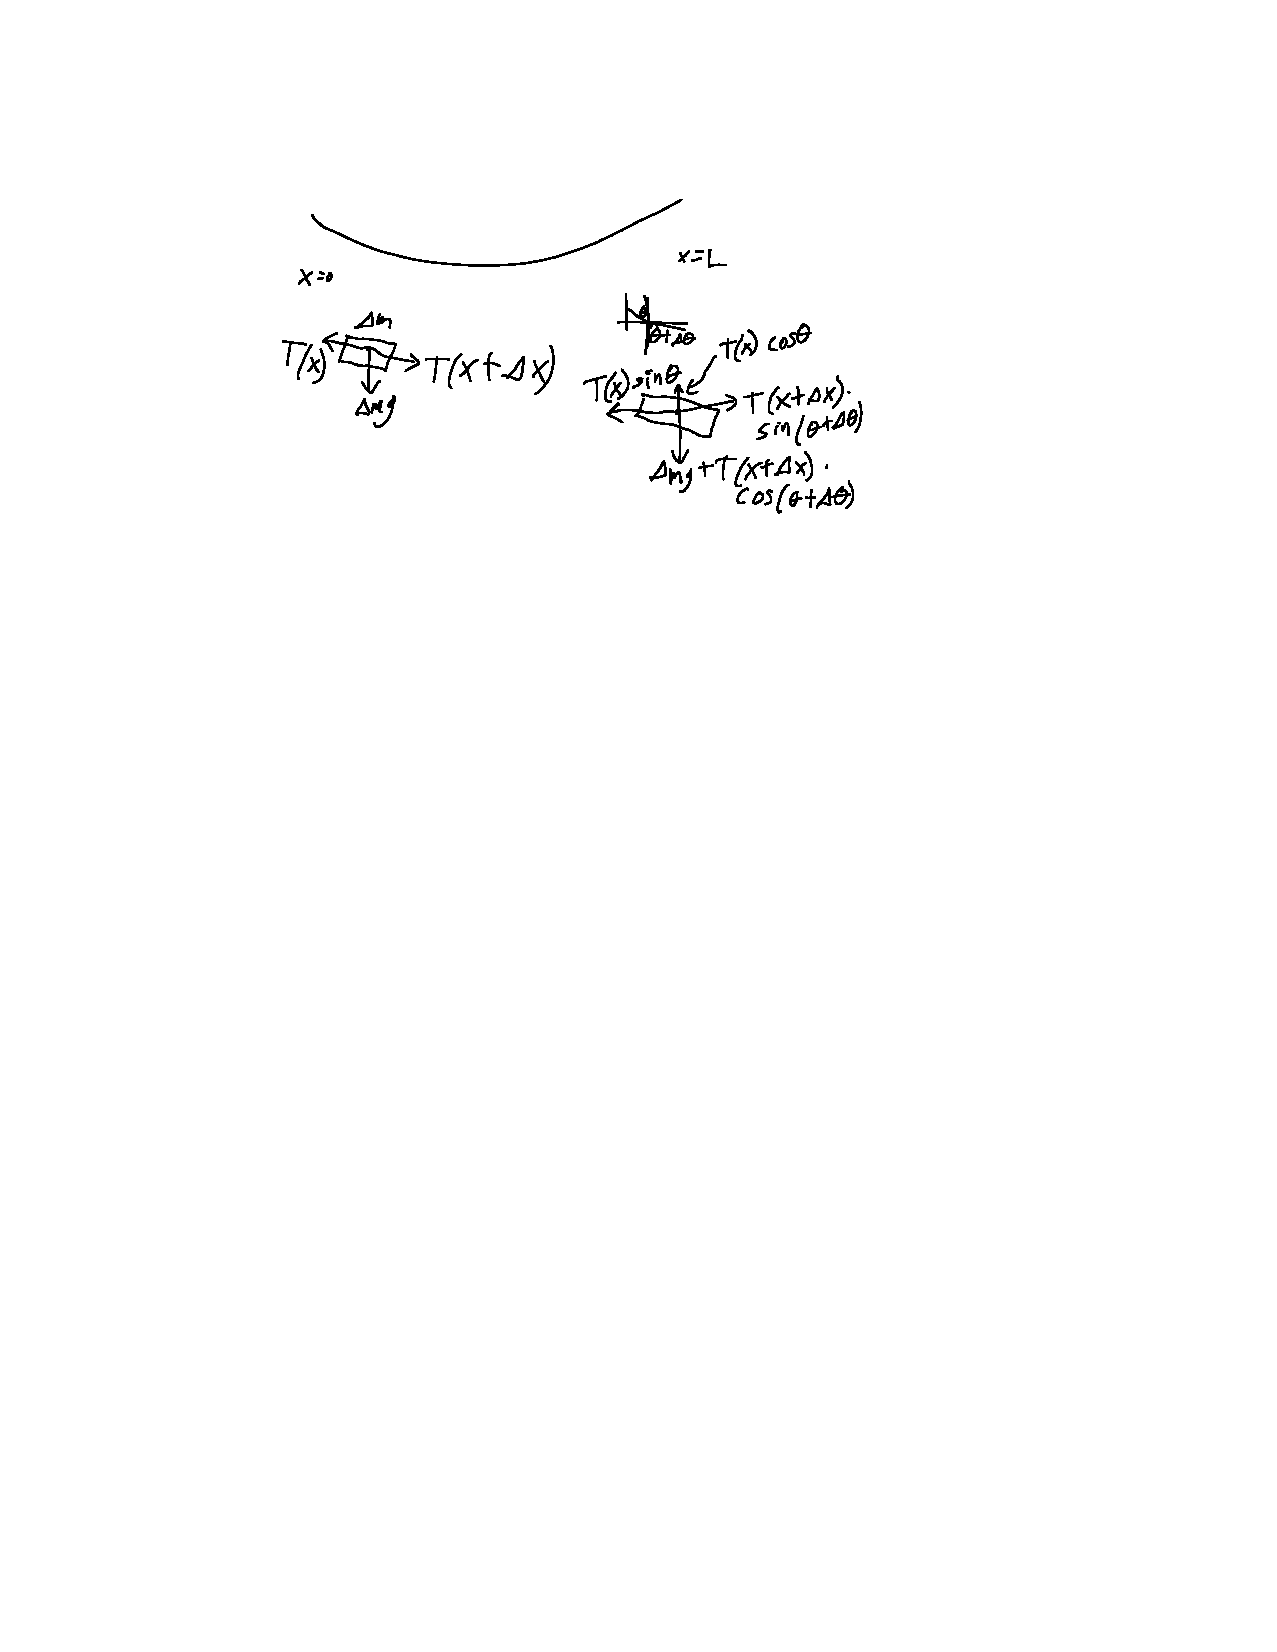
\includegraphics[width=.5\textwidth]{2009-09-25_Diagram_11_old}\end{center}  %Then \begin{align*}
%    T(x)\cos(\theta(x)) & = \Delta m g+ T(x + \Delta x)\cos(\theta(x)+\Delta\theta) \\
%    T(x)\sin(\theta(x)) & = T(x+\Delta x)\sin(\theta(x)+\Delta\theta) \\
%    \\
%    T(x + \Delta x) & = \frac{T(x)\cos(\theta(x)) - \Delta m g}{\cos(\theta(x)+\Delta\theta)} \\
%    T(x + \Delta x) & = \frac{T(x)\sin(\theta(x))}{\sin(\theta(x)+\Delta\theta)} \\
%    \\
%    T(x) & = \frac{\Delta m g+ T(x + \Delta x)\cos(\theta(x)+\Delta\theta)}{\cos(\theta(x))} \\
%    T(x) & = \frac{T(x+\Delta x)\sin(\theta(x)+\Delta\theta)}{\sin(\theta(x))} \\
%    \\
%    T(x+\Delta x) - T(x) & = T(x+\Delta x)\left( 1 - \frac{\sin(\theta(x)+\Delta\theta)}{\sin(\theta(x))}\right) \\
%      & = T(x+\Delta x)\left( -\frac{\sin(\theta(x)+\Delta\theta) - \sin(\theta(x))}{\sin(\theta(x))}\right) \\
%    \\
%    \lim_{\Delta x \longrightarrow 0} \frac{T(x+\Delta x) - T(x)}{\Delta x} & = -\lim_{\Delta x\longrightarrow 0}\frac{T(x+\Delta x)}{\sin(\theta(x))}\lim_{\Delta x\longrightarrow 0} \frac{\sin(\theta(x)+\Delta\theta) - \sin(\theta(x))}{\Delta x} \\
%    \\
%    \frac{d}{d x} T(x) & = -\frac{T(x)}{\sin(\theta(x))}\cdot \frac{d}{d x} \sin(\theta(x)) \\
%     & = -\frac{T(x)}{\sin(\theta(x))}\cos(\theta(x))\frac{d}{d x}\theta(x) \\
%  \end{align*} FIX %Since the rope is not accelerating, the tension is uniform throughout, so $T = \frac{mg}{2\cos\theta}$.
\end{enumerate}


\section*{Catenary Problem}
\begin{center}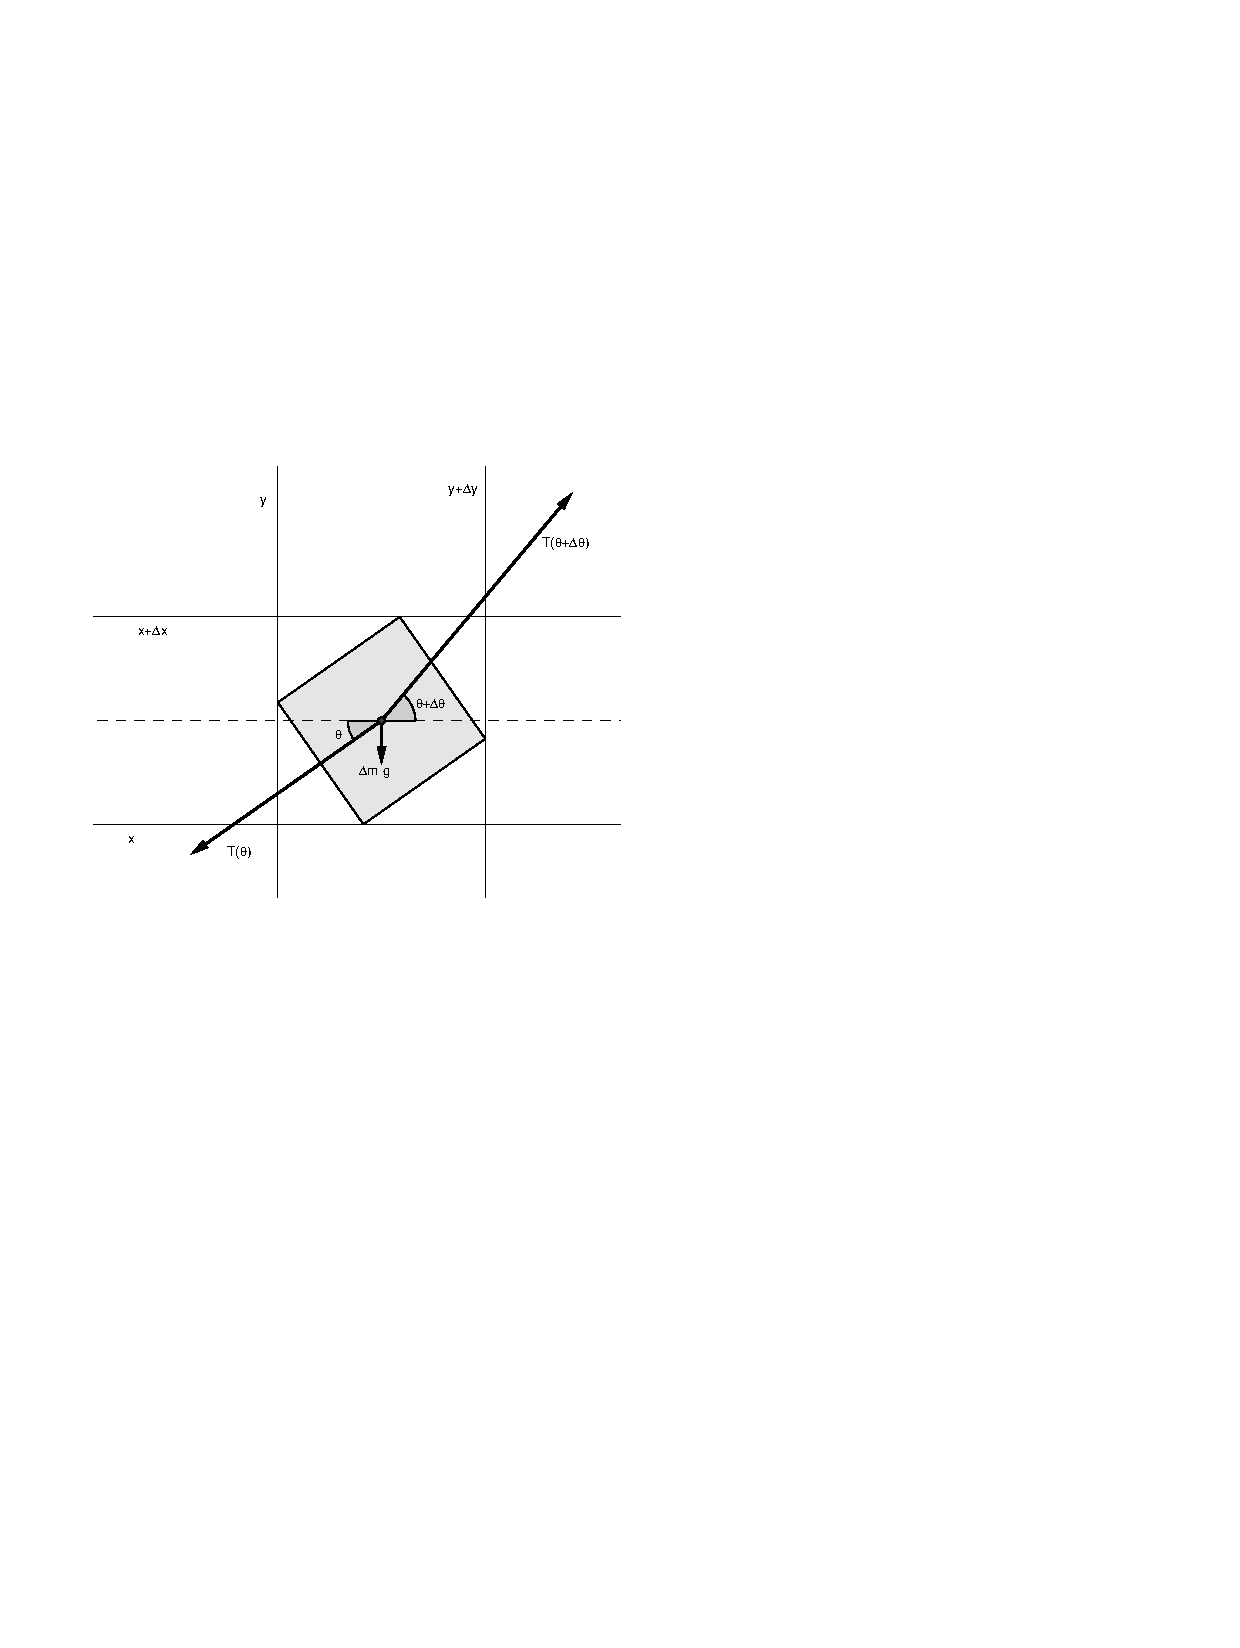
\includegraphics[width=.5\textwidth]{2009-09-25_Diagram_14}\end{center}

\begin{align*}
  T(\theta)\cos\theta & = T(\theta + \Delta \theta)\cos(\theta + \Delta \theta) \\
  %\Delta m g & = T(\theta + \Delta \theta)\sin(\theta + \Delta \theta) - T(\theta)\sin\theta \\
  \\
  T(\theta) & = \frac{T(\theta + \Delta \theta)\cos(\theta + \Delta \theta)}{\cos\theta} \\
  T(\theta) - T(\theta + \Delta\theta)& = \frac{-T(\theta + \Delta \theta)}{\cos\theta}(\cos(\theta + \Delta \theta) - \cos\theta) \\
  \\
  \lim_{\Delta\theta\rightarrow 0}\frac{T(\theta) - T(\theta + \Delta\theta)}{\Delta \theta} & = \lim_{\Delta\theta\rightarrow 0}\frac{-T(\theta + \Delta \theta)}{\cos\theta}\cdot \frac{\cos(\theta + \Delta \theta) - \cos\theta}{\Delta\theta} \\
  \frac{d}{d \theta}T(\theta) & = \frac{-T(\theta}{\cos\theta}\frac{d}{d\theta}\cos\theta \\
  \frac{d T}{d \theta} & = T(\theta)\tan\theta \\
  T(\theta) = c\sec \theta \\
  \\
  \\
\end{align*}








\begin{problem}{Fermi Problem (This problem is hard and should be a challenge.)}
  The two blocks shown in the figure are connected by a string of negligible mass. If the system is released from rest, find how far the block of mass $m_1$ slides in time $t$. Neglect friction.
\begin{center}\includegraphics{2009-09-25_ps02_1}\end{center}
\end{problem}% note that having no space at the beginning of this line is IMPORTANT
\begin{solution}
  Pressure at bottom of ocean?  Force / Area.  $(7.5\cdot 10^{21}\text{ N}) / (2.7 \cdot 10^{13}\text{ m}^2) \approx 3 \cdot 10^8$ N / m$^2$
  \begin{itemize}
    \item Force: Mass $\cdot$ Acceleration (due to gravity). $(3 \cdot 10^{21}\text{ kg}) \cdot (2.5\text{m / s}^2) \approx 7.5\cdot 10^{21}$ N
      \begin{itemize}
        \item Mass: density $\cdot$ volume.  $(10^{12}\text{ kg / km}^3) \cdot (3 \cdot 10^9\text{ km}^3) \approx 3 \cdot 10^{21}$ kg
          \begin{itemize}
            \item Density: the density of ice is about the same as that of water, 1 g / cm$^3$, or $10^{12}$ kg / km$^3$
            \item Volume: The volume is the difference of the volumes of the spheres, or $\frac{4}{3}\pi (R^3 - r^3)$, or (approximating $\pi$ as 3), $4((1600\text{ km})^3 - (1600\text{ km})^3) \approx 3 \cdot 10^9$ km$^3$
          \end{itemize}
        \item Acceleration due to gravity: Since mass is linear in volume, and volume is cubic in radius, Europa has about $\frac{1}{4^3}$ the mass of earth, and since the force of gravity is linear in mass / the square of the radius, the force of gravity on Europa is about $\frac{4^2}{4^3} = \frac{1}{4}$ that on earth, so it's about 2.5 m/s$^2$  Alternatively, by dimensional analysis, the acceleration due to gravity is linear in m$^{-1}$, so the acceleration due to gravity on Europa is about $\frac{1}{4}$ that of earth.
      \end{itemize}
    \item Area: $4\pi r^2$.  Let $\pi \approx 3$, so area is about $2.7 \cdot 10^{13}$ m$^2$
      \begin{itemize}
        \item Radius: $\frac{1}{4}$ radius of earth, less 100 km, so about 1500 km (since, according to google, the radius of earth is 6378.1 km)
      \end{itemize}
  \end{itemize}

  Alternatively:
  Pressure $ = \frac{F}{A} = \frac{mg}{A} = \frac{\rho Vg}{A} = \frac{\rho h A g}{A} = \rho h g = (10^{12}\text{ kg / km}^3)(100\text{ km})(2.5\text{ m / s}^2) \approx 3\cdot 10^8$ N / m$^2$
  \begin{itemize}
    \item Density: the density of ice is about the same as that of water, 1 g / cm$^3$, or $10^{12}$ kg / km$^3$
    \item Height: the height is about 100 km
    \item Acceleration due to gravity: Since mass is linear in volume, and volume is cubic in radius, Europa has about $\frac{1}{4^3}$ the mass of earth, and since the force of gravity is linear in mass / the square of the radius, the force of gravity on Europa is about $\frac{4^2}{4^3} = \frac{1}{4}$ that on earth, so it's about 2.5 m/s$^2$  Alternatively, by dimensional analysis, the acceleration due to gravity is linear in m$^{-1}$, so the acceleration due to gravity on Europa is about $\frac{1}{4}$ that of earth.
  \end{itemize}
\end{solution}% note that having no space at the beginning of this line is IMPORTANT

\begin{problem}{Kinematics-One Dimension}
  A bus leaves a stop at MIT and accelerates at a constant rate for 5 seconds. During this time the
  bus traveled 25 meters. Then the bus traveled at a constant speed for 15 seconds. Then the driver
  noticed a red light 18 meters ahead and slams on the brakes. Assume the bus decelerates at a
  constant rate and comes to a stop some time later just at the light.
  \begin{enumerate}[a)]
    \item What was the initial acceleration of the bus?
    \item What was the velocity at the bus after 5 seconds?
    \item What was the braking acceleration of the bus? Is it positive or negative?
    \item How long did the bus brake?
    \item What was the distance from the bus stop to the light?
    \item Make a graph of the position vs. time for the entire trip.
    \item Make a graph of the velocity vs. time for the entire trip.
    \item Make a graph of the acceleration vs. time for the entire trip.
  \end{enumerate}
\end{problem}
\begin{solution}
  \begin{enumerate}[a)]
    \item Since $\displaystyle \int_{0}^{5}\int_{0}^{t} a \d{t'}\d{t} = 25\ \text{m}$, $\frac{1}{2}a \cdot 5^2 = 25$, so $2$ m / s$^2$.
    \item 10 m / s
    \item $\frac{1}{2}at^2 = 18$ m, and $at = 10$ m / s, so $t = 3.6$ s, and $a = 2.\overline{7}$ m / s$^2$.  It is negative.
    \item 3.6 s
    \item $25 + 10 \cdot 15 + 18 = 193$ m
    \item 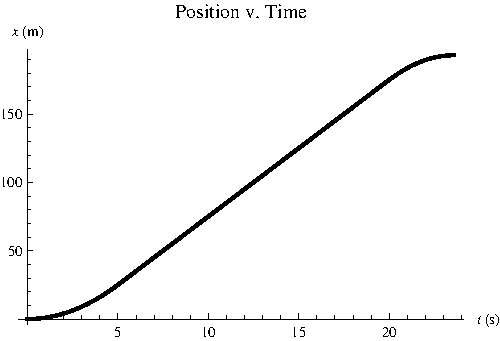
\includegraphics[width=0.85\textwidth]{ps01_Plot_1}
    \item 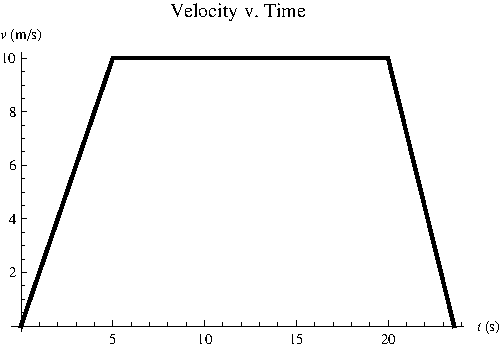
\includegraphics[width=0.85\textwidth]{ps01_Plot_2}
    \item 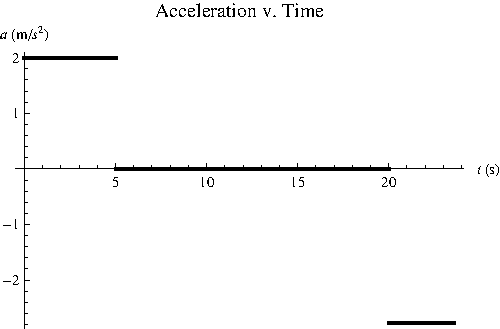
\includegraphics[width=0.85\textwidth]{ps01_Plot_3}
  \end{enumerate}
\end{solution}

\begin{problem}{Kinematics-One Dimension}
  You are a running as fast as you can at a constant velocity, $v_p$, trying to catch a bus that is at rest
  at a bus stop. When you are still a distance $b$ away from the bus stop, the bus starts to accelerate
  at a constant rate $a_\text{bus}$.
  \begin{enumerate}[a)]
    \item What is the minimum velocity that you need to run at in order to just catch the bus?
    \item Draw graphs showing the motion of the bus and yourself.
    \item How long did it take to catch the bus?
  \end{enumerate}
\end{problem}
\begin{solution}
  \begin{enumerate}[a)]
    \item If you just catch the bus after time $t$, then $v_p = a_{bus}t$.  If you catch the bus after time $t$, $v_p t = b + \frac{1}{2}a_{bus}t^2 = b + \frac{1}{2}v_p t$, so $t = \sqrt{2\frac{b}{a_{bus}}}$.  Then $v_p = \sqrt{2 b a_{bus}}$.
    \item 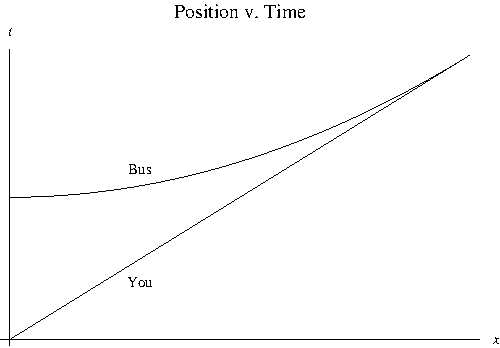
\includegraphics[width=0.85\textwidth]{ps01_Plot_4}
    \item $\sqrt{2\frac{b}{a_{bus}}}$
  \end{enumerate}
\end{solution}

\begin{problem}{K\&K 1.7}
  Let $\uvec a$ and $\uvec b$ be unit vectors in the $xy$ plane making angles $\theta$ and $\phi$ with the $x$ axis,
  respectively. Show that $\uvec a = \cos\theta\uvec i + \sin\theta\uvec j$, $\uvec b = \cos\phi\uvec i + \sin\phi\uvec j$, and using vector algebra prove
that $\cos(\theta -\phi ) = \cos\theta \cos\phi + \sin\theta \sin\phi$.
\end{problem}
\begin{solution}
  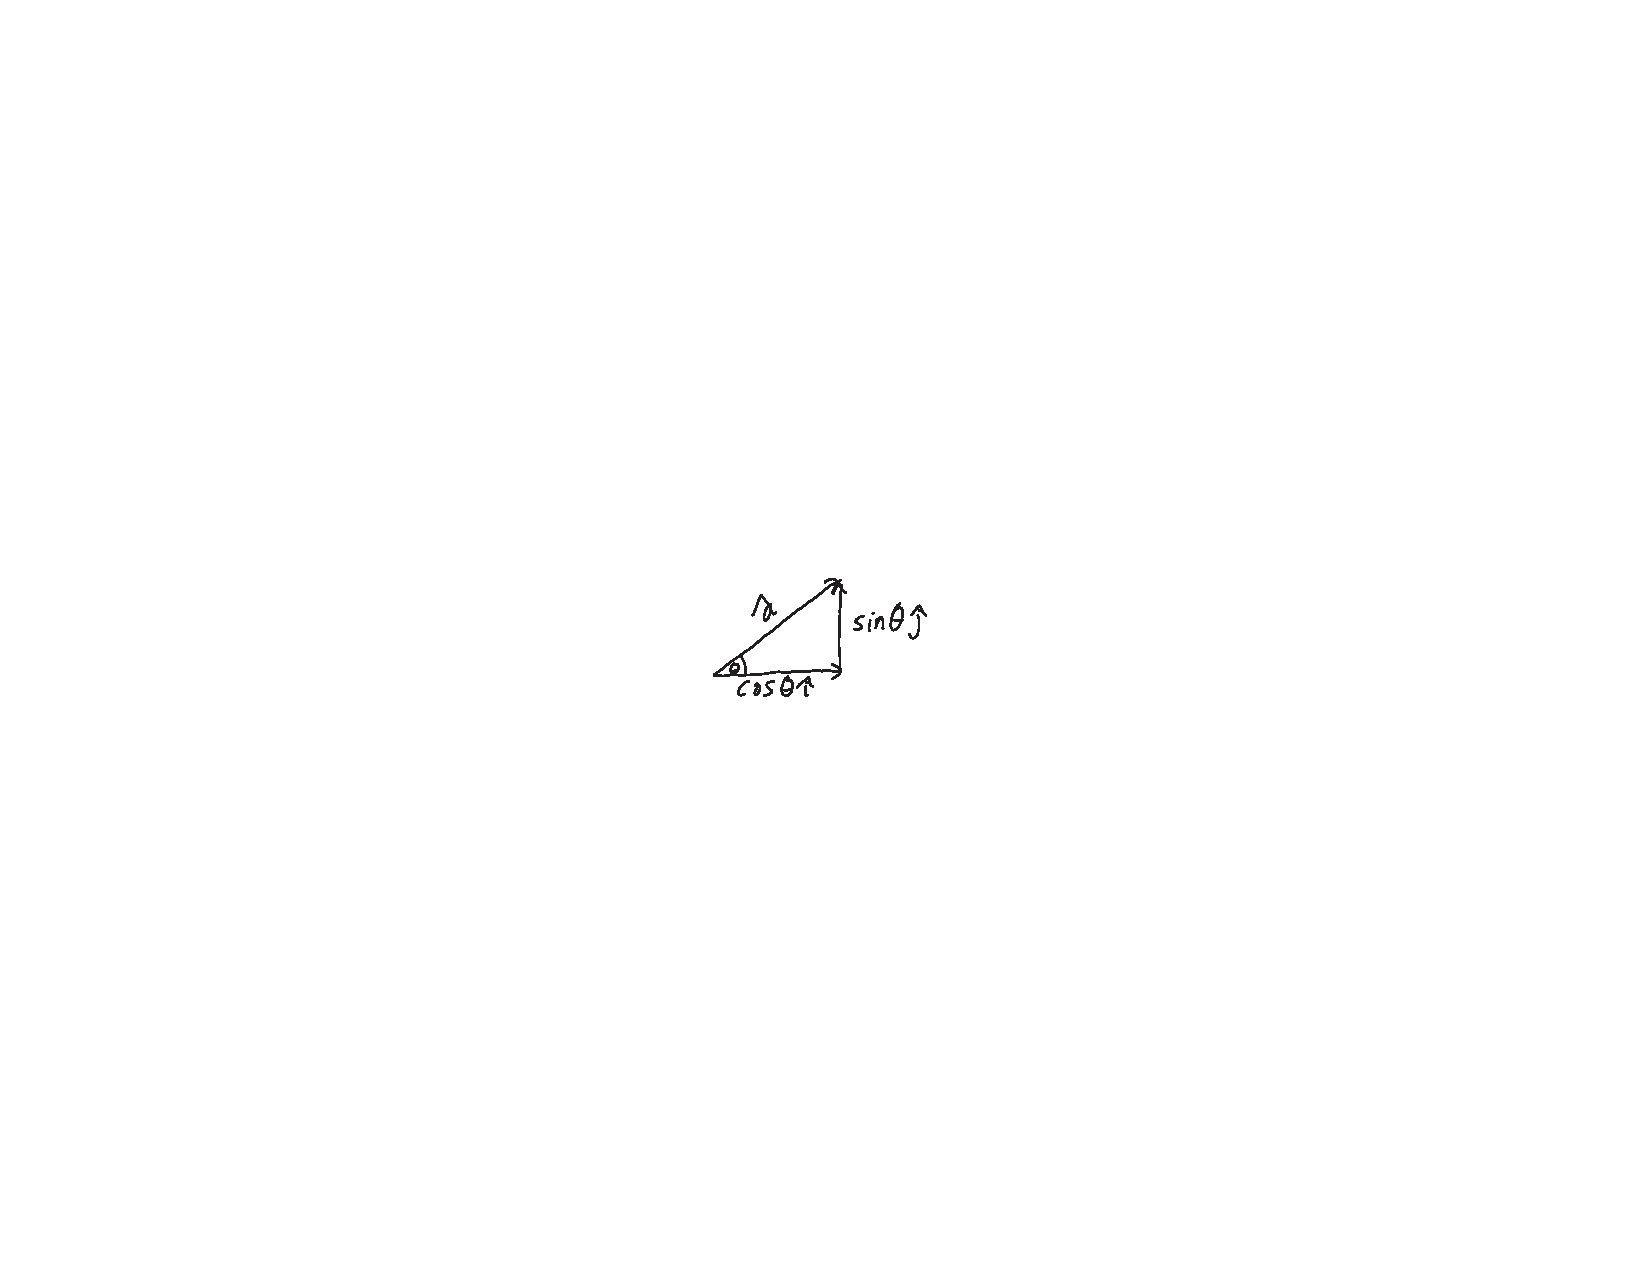
\includegraphics[width=0.85\textwidth]{ps01_Diagram_1}

  As seen in the diagram, by the definition of $\cos$ and $\sin$, $\uvec a = \cos\theta\uvec i + \sin\theta\uvec j$.  By relabeling, $\uvec b = \cos\phi\uvec i + \sin\phi\uvec j$.
  \begin{center}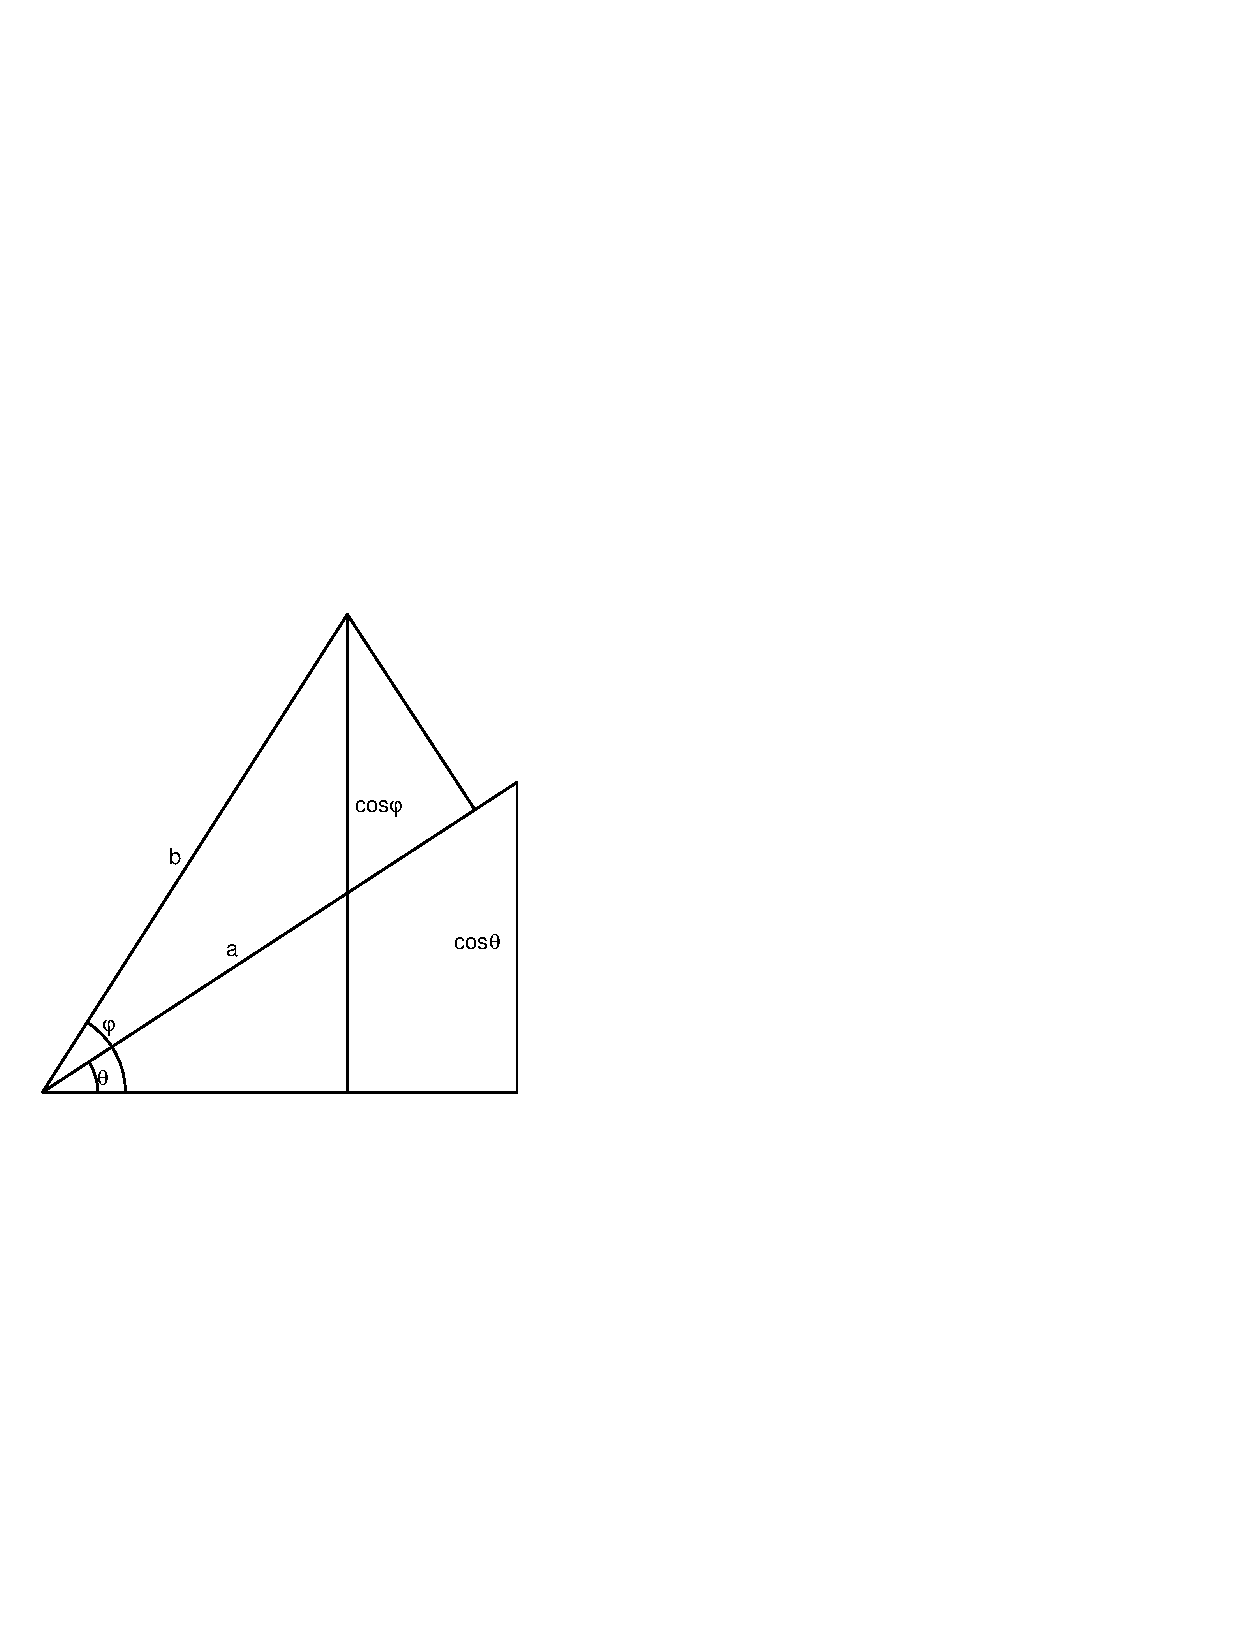
\includegraphics[width=.33\textwidth]{ps01_Diagram_2}\end{center}

  By the definition of $\cos$, $\cos(\phi - \theta) = \vec a \cdot \vec b$ (since $\vec a$ and $\vec b$ are unit vectors).  Then $\cos(\theta - \phi) = \cos(\phi - \theta) = \cos\theta\cos\phi + \sin\theta\sin\phi$.
\end{solution}

\begin{problem}{K\&K 1.12}
  The acceleration of gravity can be measured by projecting a body upward and measuring the
  time that it takes to pass two given points in both directions. Show that if the time the body takes
  to pass a horizontal line $A$ in both directions is $T_A$ , and the time to go by a second line $B$ is $T_B$,
  then, assuming that the acceleration is constant, its magnitude is
  $$g = \frac{8h}{T_A^2 - T_B^2}$$
  \begin{center}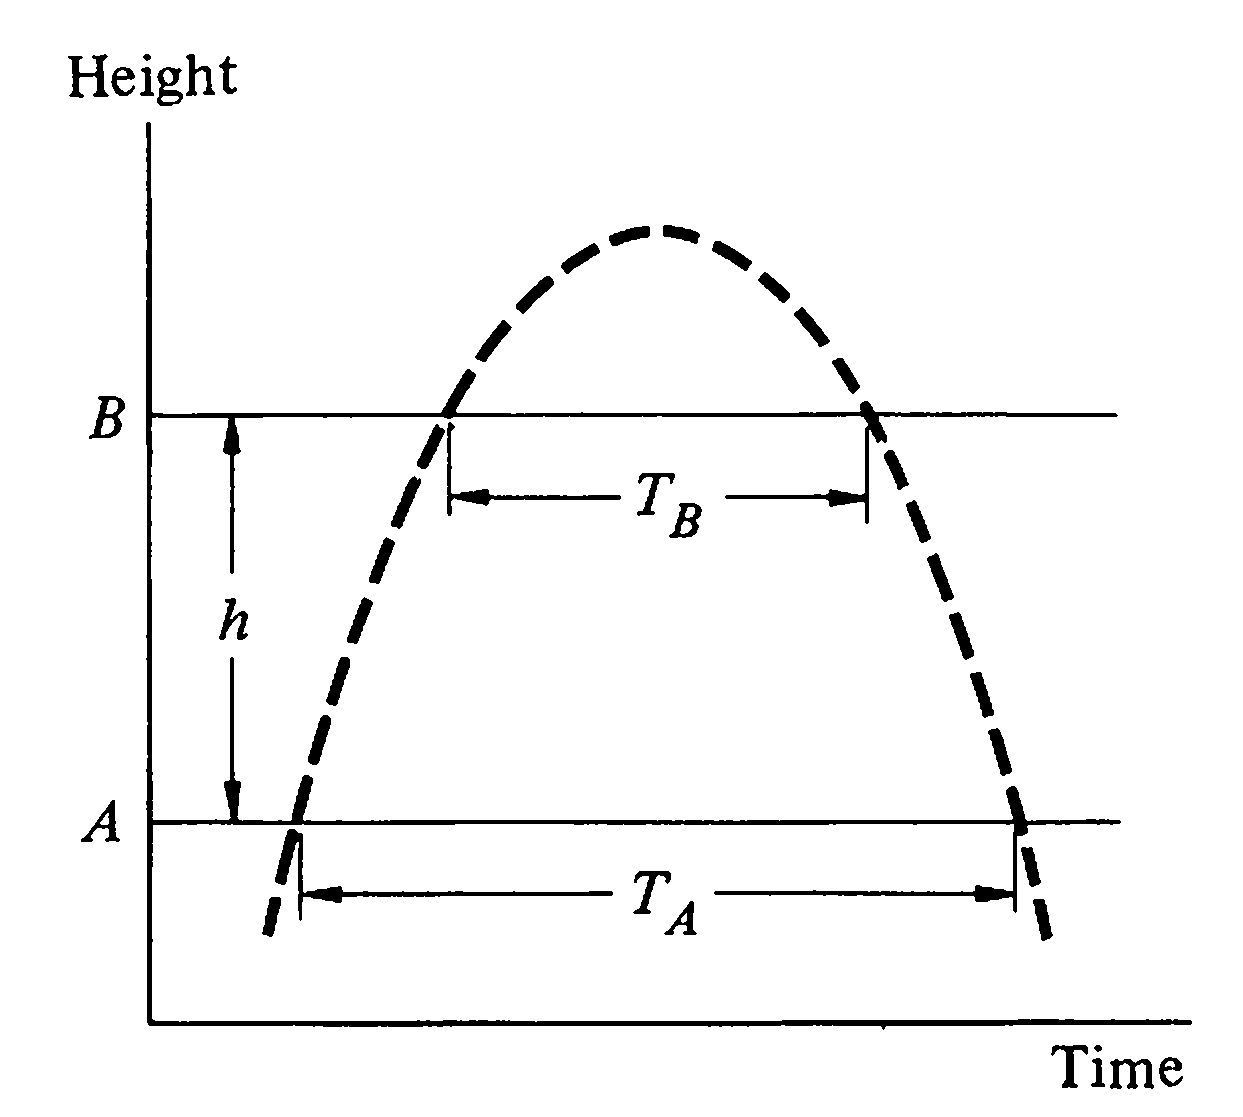
\includegraphics[width=0.35\textwidth]{ps01_1}\end{center}
\end{problem}
\begin{solution}
  Since acceleration is constant downwards, $\frac{\partial^2 y}{\partial t^2} = g$.  Then $y(t) = y_0 + v_0 t + \frac{1}{2} g t^2$.  It is given that for some $t$, $y\left(t + \frac{T_B}{2}\right) = y\left(t - \frac{T_B}{2}\right)$, and $y\left(t + \frac{T_A}{2}\right) - y\left(t + \frac{T_B}{2}\right) = h$.  Translate the function such that this $t = 0$.  Then $v_0 \frac{T_B}{2} + \frac{1}{2} g \left(\frac{T_B}{2}\right)^2 = -v_0 \frac{T_B}{2} + \frac{1}{2} g \left(\frac{T_B}{2}\right)^2$.  Equivalently, $v_0 = 0$.

  Then, the other conditions states that $\frac{1}{2} g\left(\left(\frac{T_A}{2}\right)^2 - \left(\frac{T_B}{2}\right)^2\right) = h$.  Solving for $g$, $g = \frac{8h}{T_A^2 - T_B^2}$.
\end{solution}

\begin{problem}{K\&K 1.15}
  By relative velocity we mean velocity with respect to a specified coordinate system. (The term
  velocity, alone, is understood to be relative to the observer's coordinate system.)
  \begin{center}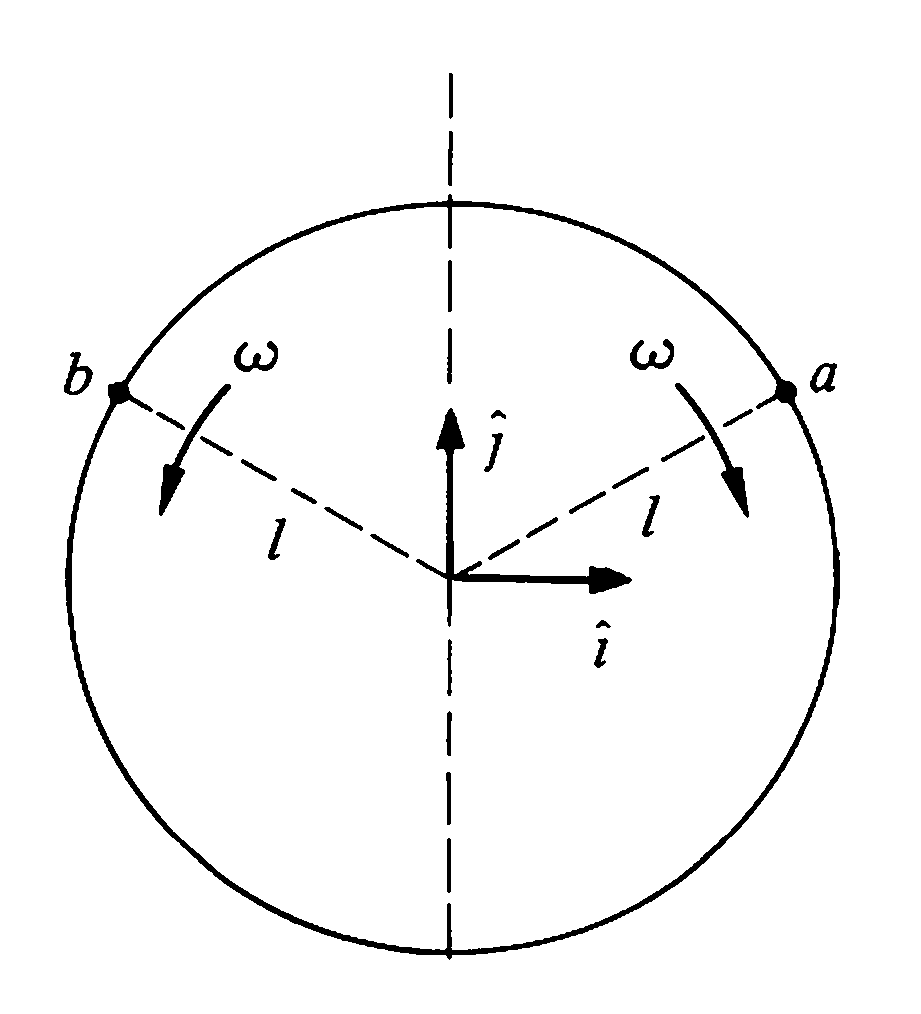
\includegraphics[width=0.35\textwidth]{ps01_2}\end{center}
  \begin{enumerate}[a.]
    \item A point is observed to have velocity $\vec v_A$ relative to coordinate system $A$. What is its
  velocity relative to coordinate system $B$, which is displaced from system $A$ by distance $\vec R$? ($\vec R$ can change in time.)
    \item Particles $a$ and $b$ move in opposite directions around a circle with angular velocity $\omega$,
  as shown. At $t = 0$ they are both at the point $\vec r = l\hat j$, where $l$ is the radius of the circle.
  Find the velocity of $a$ relative to $b$.
  \end{enumerate}
\end{problem}
\begin{solution}
  \begin{enumerate}[a.]
    \item The position vectors are related by $$\vec r_B = \vec r_A - \vec R.$$  Then velocities are related by the taking derivatives, (law of addition of velocities) $$\vec v_B = \vec v_A - \vec V.$$  %Assuming $\left\| \vec v_A\right\|$ and $\left\| \frac{\partial \vec R}{\partial t} \right\|$   are negligible compared to $c$, the velocity relative to coordinate system $B$ is $\frac{\partial\vec v_A}{\partial t} - \frac{\partial \vec R}{\partial t}$.
    \item Let's choose two reference frames; frame B is centered at particle b, and frame A is centered at the center of the circle in the figure below.
    \begin{center}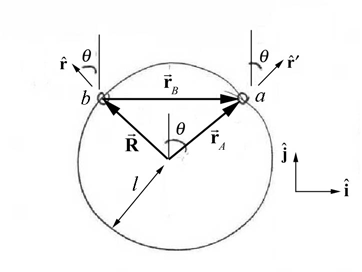
\includegraphics{ps01_Solution_06_01}\end{center}
    Then the relative position vector between the origins of the two frames is given by 
    \begin{equation*} \vec R = l\har r.\end{equation*}
    The position vector of particle a relative to frame A is given by
    \begin{equation*} \vec r_A = l\vec r'. \end{equation*}
    The position vector of particle b in frame B can be found by substituting Eqs. (1.4) and (1.3) into
Eq. (1.1),
??B A r = r ?R = l r? ? l r
? ? ? . (1.5)
We can decompose each of the unit vectors ? and ? r with respect to the Cartesian unit vectors ?
and ? (see figure)
r?= ?sin? ? + cos? ? (1.6)
r? = sin? ? + cos? ? . (1.7)
Then Eq. (1.5) giving the position vector of particle b in frame B becomes
??(sin ?cos ? ( sin ?cos ? 2 sin ?B r? = l r? ? l r = l ? i + ? j ? l ? ? i + ? j = l ? i . (1.8)
In order to find the velocity vector of particle a in frame B (i.e. with respect to particle b),
differentiate Eq. (1.8)
(2 sin ) ?(2 cos ) ?2 cos ?B
        $\vec a = l\hat r_a$, $\vec b = l\hat r_b$.  %The velocity of $a$ relative to $b$, $\vec a_b$, is $\frac{\partial\vec v_A}{\partial t} - \frac{\partial \vec b}{\partial t} = l\left(\frac{\partial\hat r_a}{\partial t} - \frac{\partial \hat r_b}{\partial t}\right)$.  Since it is circular motion, $\frac{\partial \hat r_a}{\partial t} = -\omega\hat\theta$ and $\frac{\partial \hat r_b}{\partial t} = \omega\hat\theta$.  Then $\vec a_b = -2l\omega\hat\theta = 2 l \omega \cos(\omega t)\hat i$. \par Equivalently, 
    $\hat r_a = \cos(\omega t)\hat j + \sin(\omega t)\hat i$ and $\hat r_b = \cos(\omega t)\hat j -\sin(\omega t)\hat i$.  The velocity of $a$ relative to $b$, $\vec a_b$, is $\frac{\partial\vec v_A}{\partial t} - \frac{\partial \vec b}{\partial t} = l\left(\frac{\partial\hat r_a}{\partial t} - \frac{\partial \hat r_b}{\partial t}\right)$.  Since it is circular motion, $\frac{\partial \hat r_b}{\partial t} = -\omega(\sin(\omega t)\hat j + \cos(\omega t)\hat i)$ and $\frac{\partial \hat r_a}{\partial t} = \omega(-\sin(\omega t)\hat j + \cos(\omega t)\hat i)$.  Then $\vec a_b = l\omega\left(-\sin(\omega t)\hat j + \cos(\omega t)\hat i + \sin(\omega t)\hat j + \cos(\omega t)\hat i\right) = 2 l \omega \cos(\omega t)\hat i$.
  \end{enumerate}
\end{solution}

\begin{problem}{K\&K 1.19}
  A bicycle wheel of radius $a$ is rolling in a straight line without slipping at a constant horizontal
  velocity $V$. A bead is fixed to a spoke a distance $b$ from the center of the wheel.
  \begin{center}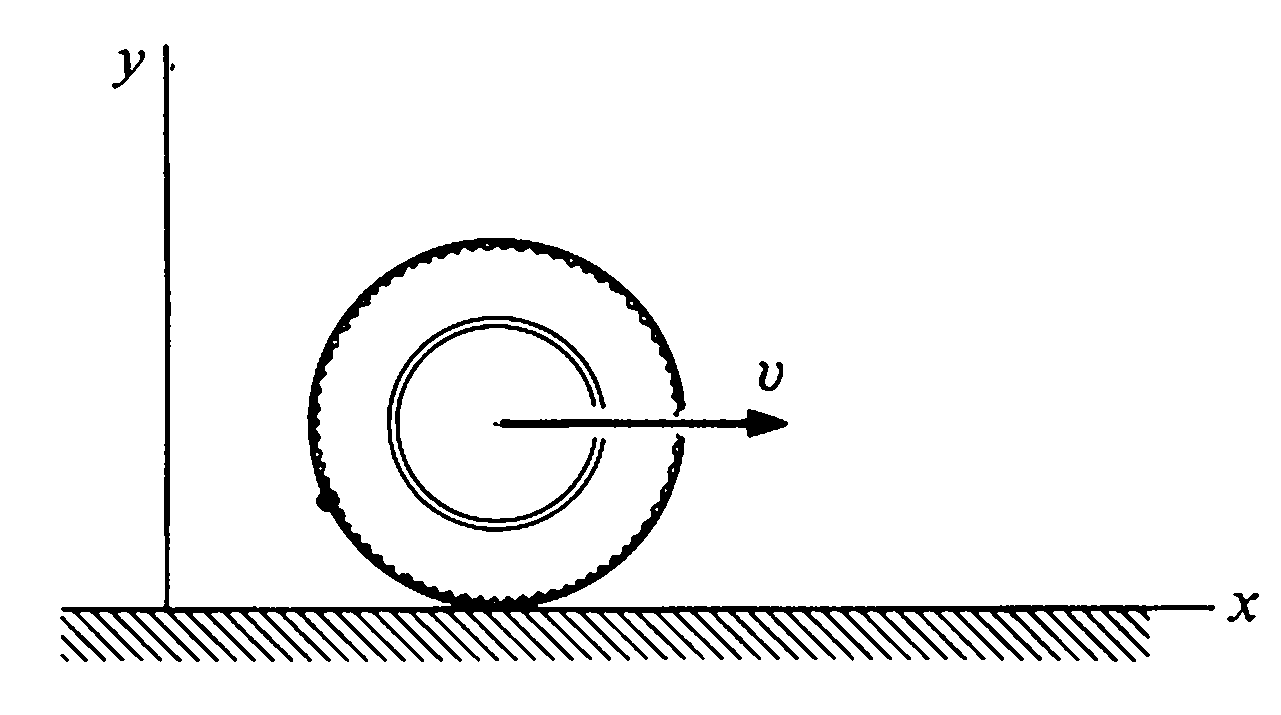
\includegraphics[width=0.5\textwidth]{ps01_3}\end{center}
  \begin{enumerate}[a)]
    \item Find the position and velocity of the bead as a function of time as seen by an observer located
  at the center of the wheel and moving with the wheel. Make sure you use appropriate unit
  vectors in your answer.
    \item What is the position and velocity of the observer at the center of the wheel as seen by an
  observer fixed to the ground. Assume at $t = 0$ that the center of the wheel is directly over the
  observer fixed to the ground. Make sure you use appropriate unit vectors in your answer.
    \item What is the relation between the angular velocity of the wheel, $\omega$, and the horizontal velocity, $V$, of the wheel?
    \item Find the position and velocity of the bead as a function of time as seen by the observer fixed
  to the ground. Make sure you use appropriate unit vectors in your answer.
  \end{enumerate}
\end{problem}
\begin{solution}
  \begin{enumerate}[a)]
    \item The angular velocity of the wheel, $\omega = 2\pi \frac{V}{2\pi a} = \frac{V}{a}$.  Then the position of the bead is given by $\vec r = b\cos\left(\frac{V}{a}t\right)\hat i + b\sin\left(\frac{V}{a}t\right)\hat j$.  $\frac{\partial \vec r}{\partial t} = -b\frac{V}{a}\sin\left(\frac{V}{a}t\right)\hat i + b\frac{V}{a}\cos\left(\frac{V}{a}t\right)\hat j$
    \item $\frac{\partial \vec x}{\partial t} = V\hat i$ and $\vec x = V t\hat i$
    \item $\omega = 2\pi \frac{V}{2\pi a} = \frac{V}{a}$
    \item $\vec r_G = \left(b\cos\left(\frac{V}{a}t\right) + Vt\right)\hat i + b\sin\left(\frac{V}{a}t\right)\hat j$ and $\frac{\partial \vec r_G}{\partial t} = \left(-b\frac{V}{a}\sin\left(\frac{V}{a}t\right) + V\right)\hat i + b\frac{V}{a}\cos\left(\frac{V}{a}t\right)\hat j$
  \end{enumerate}
\end{solution}

\begin{problem}{K\&K 1.20}
  A particle moves outward along a spiral. Its trajectory is given by
  $r = A\theta$, where $A$ is a constant, $A = (1/\pi )$ m $\cdot$ rad$^{-1}$.  $\theta$ increases in time according to $\theta =\alpha t^2 / 2$, where $\alpha$ is a constant.
  \begin{enumerate}[a.]
    \item Sketch the motion, and indicate the approximate velocity and acceleration at a few
  points.
    \item Show that the radial acceleration is zero when $\theta =1/\sqrt{2}$ rad.
    \item At what angles do the radial and tangential accelerations have equal magnitude?
  \end{enumerate}
\end{problem}
\begin{solution}
  \begin{enumerate}[a.]
    \item 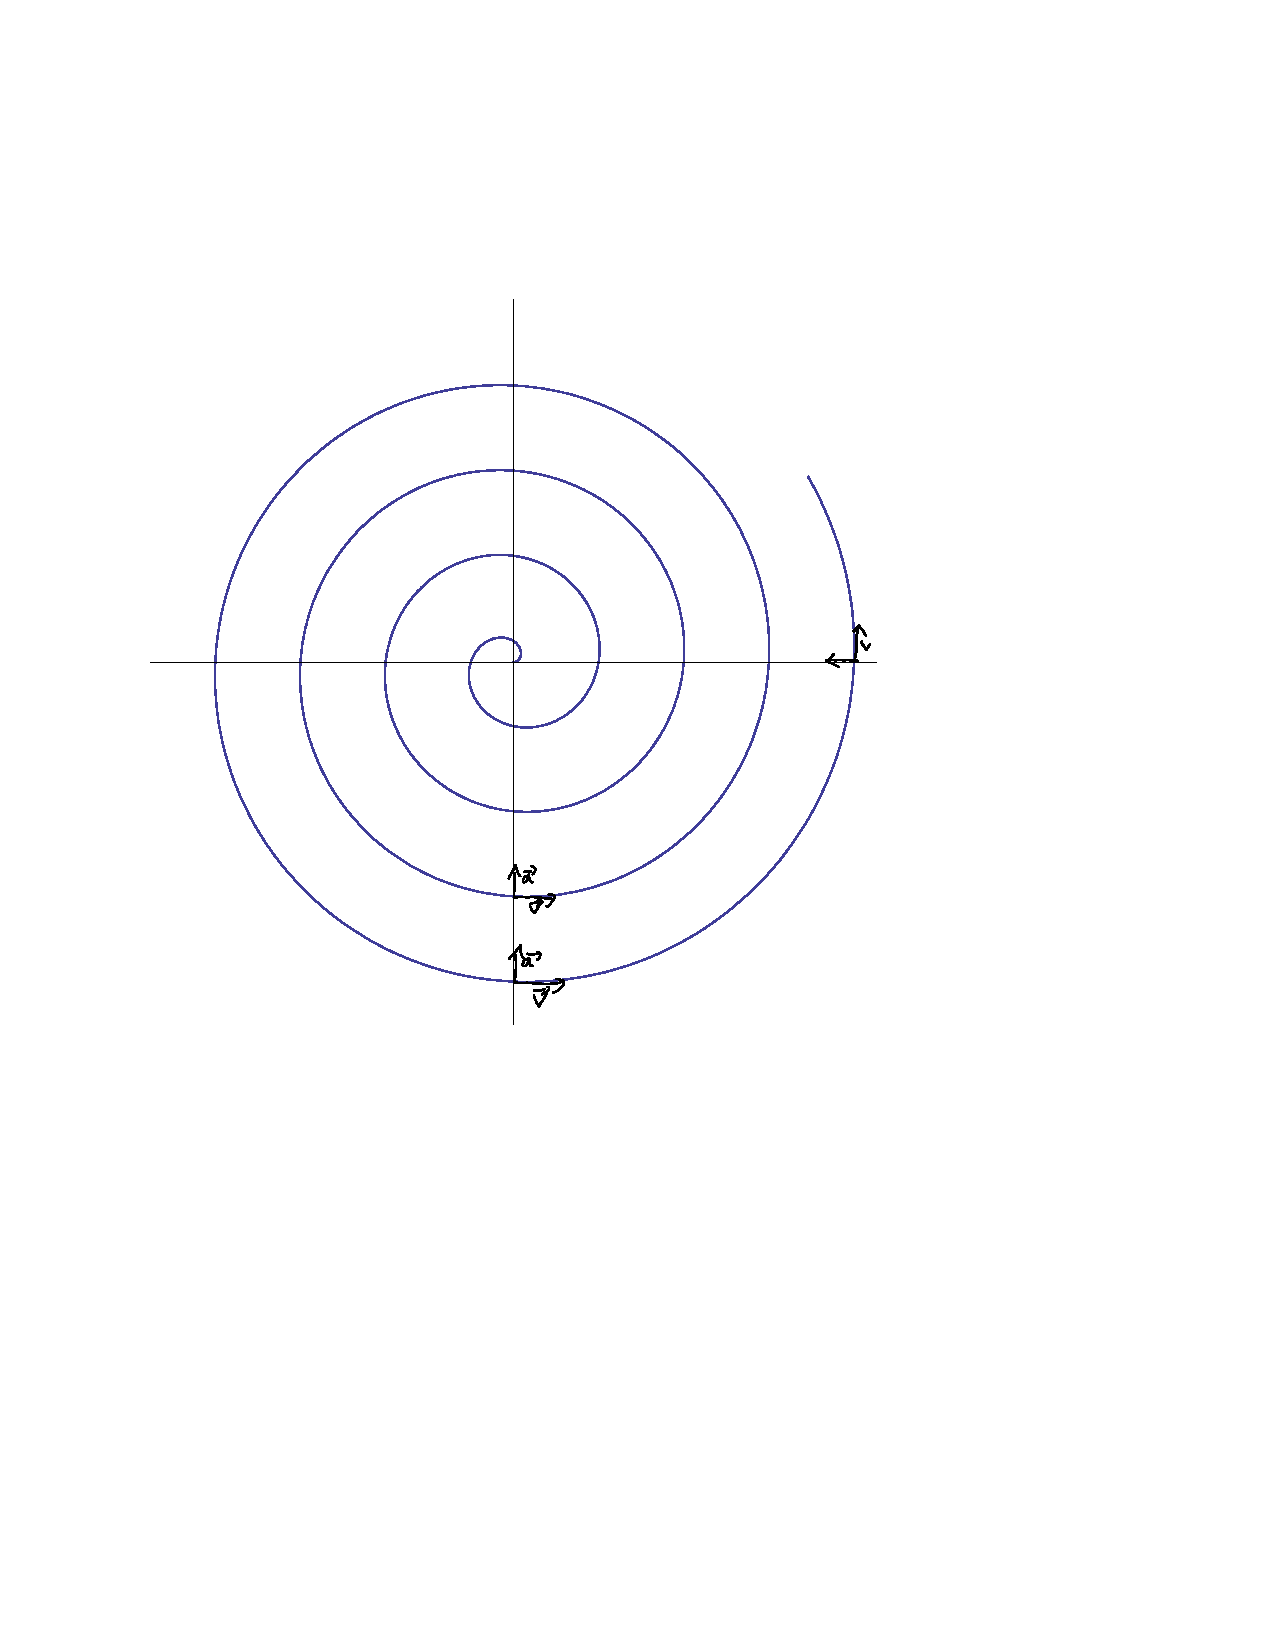
\includegraphics[width=0.85\textwidth]{ps01_Diagram_3}
    \item \begin{align*}
            \vec r(t) & = A\frac{\alpha t^2}{2} \hat r \\
            \vec \theta(t) & = \frac{\alpha t^2}{2} \hat\theta \\
            \\
            \frac{\partial \hat r}{\partial t} & = \alpha t \hat \theta \\
            \frac{\partial \hat \theta}{\partial t} & = -\alpha t \hat r \\
            \\
            \frac{\partial \vec r}{\partial t} & = \frac{A\alpha}{2}\left( 2t\hat r + t^2\frac{\partial \hat r}{\partial t}\right) \\
            & = \frac{A\alpha}{2}\left( 2t\hat r + \alpha t^3 \hat \theta\right) \\
            \\
            \frac{\partial^2 \vec r}{\partial t^2} & = \frac{A\alpha}{2}\frac{\partial}{\partial t}\left( 2t\hat r + \alpha t^3 \hat \theta\right) \\
            & = \frac{A\alpha}{2}\left( 2\hat r + 2t\frac{\partial \hat r}{\partial t} + 3\alpha t^2 \hat \theta + \alpha t^3\frac{\partial \hat \theta}{\partial t}\right) \\
            & = \frac{A\alpha}{2}\left( 2\hat r + 2t\alpha t \hat \theta + 3\alpha t^2 \hat \theta + \alpha t^3(-\alpha t \hat r)\right) \\
            & = \frac{A\alpha}{2}\left( 2\hat r + 2\alpha t^2 \hat \theta + 3\alpha t^2 \hat \theta - \alpha^2 t^4\hat r\right) \\
            & = \frac{A\alpha}{2}\left( \left(2- 4\left(\frac{\alpha t^2}{2}\right)^2\right)\hat r + 5\alpha t^2\hat \theta \right) \\
            & = A\alpha\left( \left(1- 2\theta^2\right)\hat r + 5\theta\hat \theta \right) \\
            & = A\alpha\left( \left(1- 2\cdot\frac{1}{2}\right)\hat r + \frac{5}{\sqrt{2}}\hat \theta \right) \\
            & = \frac{5A\alpha}{\sqrt{2}}\hat \theta
          \end{align*} \par
          Since all of the coefficient of $\hat r$ is 0, the radial acceleration is 0.
    \item  The radial and tangential accelerations have equal magnitudes if $1- 2\theta^2 = 5\theta$.  That is, $\theta \equiv \frac{-5\pm\sqrt{33}}{4}\pmod{2\pi}$.
  \end{enumerate}
\end{solution}

\begin{problem}{K\&K 1.21}
  A person throws a rock from the top of a hill. The hill slopes downward uniformly at angle $\phi$. At
  what angle $\theta$ from the horizontal should the person throw the rock so that it has the greatest
  range?
  \begin{center}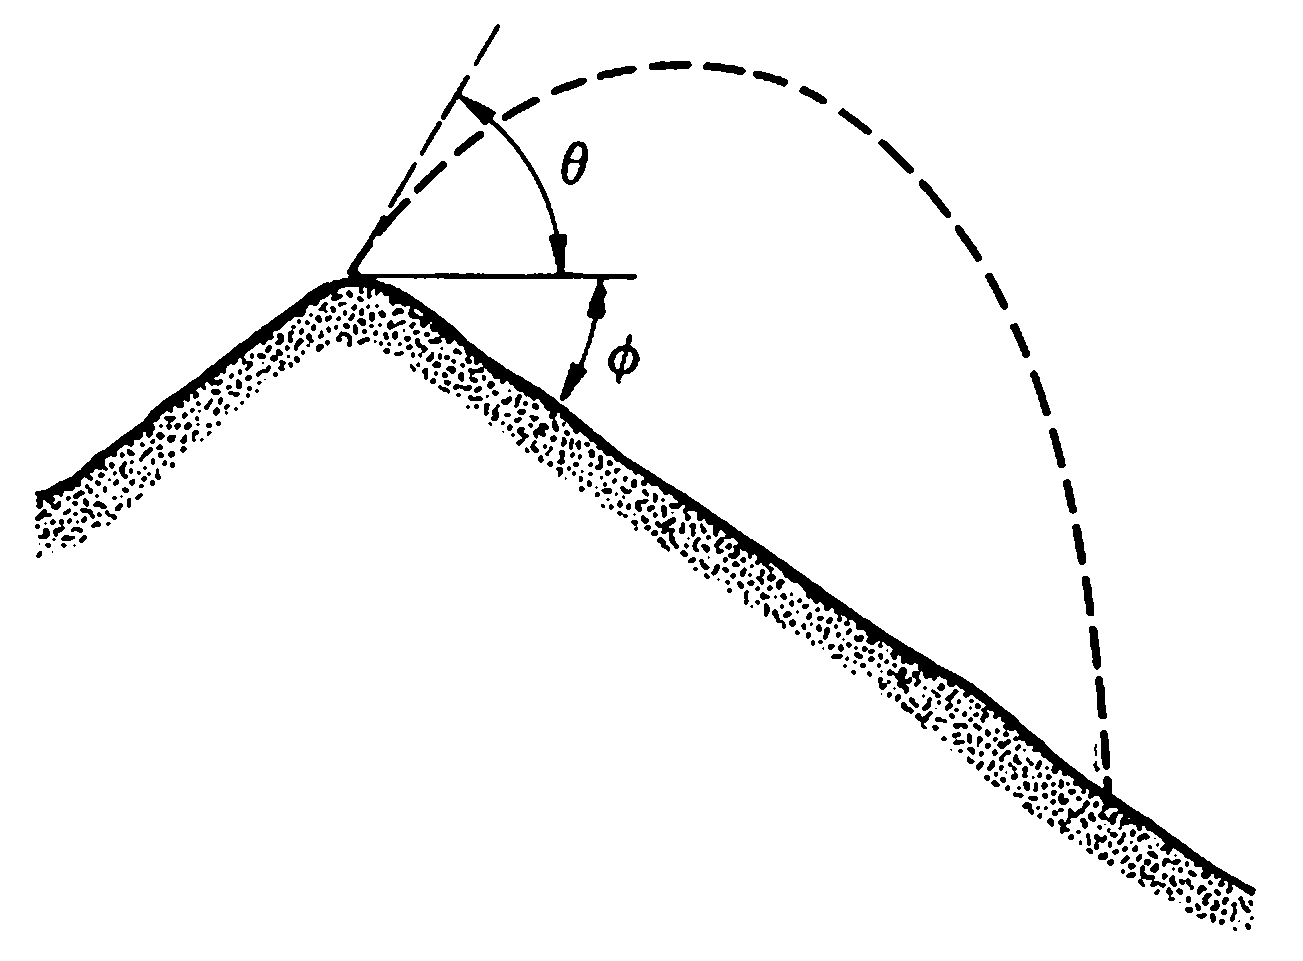
\includegraphics[width=0.5\textwidth]{ps01_4}\end{center}
\end{problem}
\begin{solution}
  The height of the hill, $h_h(x)$, is $-x\tan \phi$.  The acceleration of the rock, $\frac{\partial^2 \vec r(t)}{\partial t^2}$, is $-g\hat j$.  The velocity of the rock, $\frac{\partial \vec r(t)}{\partial t}$, is $(v_0\sin\theta -gt)\hat j + v_0\cos\theta \hat i$.  The position of the rock, $\vec r(t)$, is $\left(v_0 t\sin\theta -\frac{1}{2}gt^2\right)\hat j + v_0 t\cos\theta \hat i$.  The rock stops when $v_0 t\sin\theta -\frac{1}{2}gt^2 = -v_0 t \cos\theta\tan \phi$, or $v_0\sin\theta -\frac{1}{2}gt = -v_0 \cos\theta\tan \phi$.  Solving for $t$, $t = \frac{2v_0\sin\theta + 2v_0 \cos\theta\tan \phi}{g}$.  The maximal range occurs when $v_0 t\cos\theta = v_0 \frac{2v_0\sin\theta\cos\theta}{g} + v_0\frac{2v_0 \cos^2\theta\tan \phi}{g} = \frac{v_0^2\sin2\theta + 2v_0^2 \cos^2\theta\tan \phi}{g}$ is maximal, which occurs when $\frac{2v_0^2\cos2\theta + 4v_0^2 \cos\theta\sin\theta\tan \phi}{g} = 0$, or $\cos2\theta\cos\phi + \sin2\theta\sin \phi = \cos(\phi - 2\theta) = 0$.  This is true when $\phi - 2\theta = 2k\pi \pm \frac{\pi}{4}$ for $k\in\mathbb{Z}$.  Then, the optimal angle is $\frac{\phi}{2} - \frac{\pi}{8}$.
\end{solution}

\end{document}

